%%%%%%%%%%%%%%%%%%%%%%%%%%%%%%%%%%%%%%%%%%%%%%%%%%%%
%Dissertation template for the MSc in Statistics at the University of Sheffield
%You should not change anything between lines 4 and 39 of this file, except 
% to enter your title on line 9 and your name on line 10.
\documentclass{somasmsc}
\begin{document}
%%%%%%%%%%%%%%%%%%%%%%%%%%%%%%%%%%%%%%%%%%%%%%%%%%%%
%%%% Edit the next two lines in the obvious way %%%%
\newcommand{\yourtitle}{Small Neural Networks with Interesting Architectures}
\newcommand{\yourname}{Reg. 210138711}
%%%%%%%%%%%%%%%%%%%%%%%%%%%%%%%%%%%%%%%%%%%%%%%%%%%%

%%%%%%%%%%%%%%%%%%%%%%%%%%%%%%%%%%%%%%%%%%%%%%%%%%%%
% To add your acknowledgements and abstract
% edit (and save) the files called acknowledgements.tex and
% abstract.tex (in the current directory) and
% then compose this file using pdflatex
\include{frontpage}
\pagestyle{empty}
\frontmatter
\maketitle
\pagestyle{plain}
\tableofcontents
\newpage
\include{acknowledgements}
\include{lay_summary}

%setup some simple running headers
\setlength{\headheight}{16pt}
\fancyhead{}
\fancyfoot{}
\pagestyle{fancy}
\fancyhead[RO,LE]{\thepage}
\fancyhead[LO,RE]{\rightmark}

%setup commenting
\newcommand{\studentcomment}[1]{\todo[inline, backgroundcolor=blue!30]{\textsc{\yourname:} #1}}
\newcommand{\DSWcomment}[1]{\todo[inline, backgroundcolor=green!30]{\textsc{DSW:} #1}}
\newcommand{\supcomment}[1]{\todo[inline, backgroundcolor=red!30]{\textsc{Supervisor:} #1}}

\mainmatter

%%%%%%%%%%%%%%%%%%%%%%%%%%%%%%%%%%%%%%%%%%%%%%%%%%%%
%%%%%%%%%%%%%%%%%%%%%%%%%%%%%%%%%%%%%%%%%%%%%%%%%%%%

%%%%%%%%%%%%%%%%%%%%%%%%%%%%%%%%%%%%%%%%%%%%%%%%%%%%
% You should write the main part of your thesis below here
%%%%%%%%%%%%%%%%%%%%%%%%%%%%%%%%%%%%%%%%%%%%%%%%%%%%

\chapter{Introduction}\label{intro}

\section{Neural Networks}

Artificial Neural Networks (ANNs), or simply "Neural Networks" for short, are perhaps one of the most popular and well-known class of machine learning models in the world today, able to outperform humans in a number of tasks with applications such as AlphaGo \citep{silver2016mastering}, a computer player for the game Go, and ChatGPT, a chat-bot with exceptional language capabilities that was the focus of a huge number of articles and news reports in 2023 \citep{ray2023chatgpt}. Neural networks have been widely applied in image processing, including medical image diagnostics \citep{jiang2010medical}, and finance \citep{fadlalla2001analysis}, where they are often able to outperform traditional statistical models.

Artificial Neural Networks are inspired by biological neural networks found in animal brains, which are composed of neurons connected to each other via synapses. Organized into large networks, such a system is able to process information by sending electrical signals throughout the network.

An Artificial Neural Network similarly consists of neurons and connections, which are represented in a graph of vertices (or nodes) and edges respectively. Typically, these networks are arranged into layers of nodes, where the edges connect the nodes from one layer to the nodes in an adjacent layer. The layer at the start of the network is the input layer, where the nodes take the input data, and the layer at the end of the network is the output layer, which produces the output data. The layers in between are called hidden layers. Each edge is assigned a weight, which is a real value that "scales" the information from one node to another. The weights in a network determine the relationship between the input data and the output data, and so adjusting these weights determines how well a neural network will perform at a given task. Attached to the output nodes of each layer is an activation function which is applied to the scaled input it receives.

\studentcomment{Include basic feed forward diagram example here}

\subsection{Layer Architectures}

Here we introduce different types of layers and the notation used to describe how they function. In general, a layer $\mathcal{L}$ is a function that takes an input $\pmb{x}$ from a previous layer, and produces an output $\mathcal{L}\left(\pmb{x}\right)$. We will use $\mathcal{L}^{\left[i\right]}$ to denote the $i$-th layer of a neural network. Neural network layers take real input values and produce real output values, although we will see examples where the networks are specially designed to restrict the inputs and/or outputs to integers or natural numbers.

A \textit{dense layer} or \textit{fully-connected layer} is a layer where the input and output are fully connected: every node in the input layer is connected by an edge to every node in the output layer. The output of a dense layer is calculated according to a \textit{weights matrix} $\mathbf{W}$, a \textit{bias vector} $\pmb{b}$, and an \textit{activation function} $f$. The output of a dense layer is calculated as
\begin{align*}
\mathcal{L}\left(\pmb{x}\right) = f\left(\mathbf{W}\pmb{x} + \pmb{b}\right).
\end{align*}

Note that when writing exact weights for our hand-built models, the dimensions often make it more convenient to write out $\mathbf{W}^T$ and/or $\pmb{b}^T$.

A \textit{convolutional layer} is a layer where the traditional connections of a dense layer are replaced by one or more \textit{filters} or \textit{kernels}. We will consider convolutional layers in 2 dimensions: instead of an input vector $\pmb{x}$, a 2D convolutional layer $\mathcal{L}$ receives an input matrix $\mathbf{X}$ (typically representing an image) and returns an output matrix $\mathcal{L}\left(\mathbf{X}\right)$. A kernel is a collection of weights also represented by a matrix $\mathbf{W}$. Instead of matrix multiplication, the weights are combined with the input through \textit{convolution}. A matrix $\mathbf{W}$ of size $p \times q$ convoluted with an input matrix $\mathbf{X}$ of size $n \times m$ to produce an output matrix $\mathbf{Y}$ of size $\left(n-r+1\right),\left(m-s+1\right)$ through
\begin{align*}
\left[\mathbf{Y}\right]_{i,j} = \sum_{r=0}^{p-1} \sum_{s=0}^{q-1} \left[\mathbf{X}\right]_{i+r, j+s} \left[\mathbf{W}\right]_{r,s}.
\end{align*}
The layer then adds a bias $b$ and applies an activation function $f$ elementwise, so the output of the layer is
\begin{align*}
\left[\mathcal{L}\left(\mathbf{X}\right)\right]_{i,j} = f\left(\sum_{r=0}^{p-1} \sum_{s=0}^{q-1} \left[\mathbf{X}\right]_{i+r, j+s} \left[\mathbf{W}\right]_{r,s} + b\right).
\end{align*}
For image processing, convolutional layers have some notable benefits over dense layers:
\begin{itemize}
    \item Convolution applies to entries in $\mathbf{X}$ that are spatially close to each other, which are typically closely related in the context of an image. The output of a convolution layer is often called a \textit{feature map}, with elements corresponding to specific image \textit{features} identified by the kernel.
    \item The dimensions $p,q$ of the weights matrix $\mathbf{W}$ are generally much smaller than the dimensions $n, m$ of the image $\mathbf{X}$, which we expect to be large. Therefore, a convolutional layer adds far fewer parameters to the model than would be required to perform matrix multiplication on the image $\mathbf{X}$, reshaped into a vector of size $nm$.
    \item As a single kernel adds relatively few parameters to the model, convolutional layers can easily be expanded by adding additional kernels to explore and learn additional features. A convolutional layer with multiple kernels evaluated simultaneously can be referred to as having multiple \textit{channels}.
\end{itemize}

Often used in conjunction with convolutional layers, a \textit{max pooling layer} is a layer that takes and image or feature map $\mathbf{X} \in \mathbb{R}^{n \times m}$ and returns an output matrix $\mathcal{L}\left(\mathbf{X}\right) \in \mathbb{R}^{u \times v}$, where $u < n$ and $v < m$. The max pooling layer takes a sub-matrix of size $p \times q$ of $\mathbf{X}$ and returns the maximum element. The purpose of a max pooling layer is to reduce the size of the output from a convolutional layer, as this is usually similar in size to that of the original image, whilst retaining the most relevant information. We will consider max pooling where each sub-matrix that pooling is applied to does not overlap, so the expected output will be of size $n/p \times m/q$. If $u$ or $v$ does not divide $n$ or $m$ respectively, the input may be \textit{padded} with zeros so that the output is of size $\lceil n/p \rceil \times \lceil m/q \rceil$. Max pooling is applied to each channel from the convolutional layer, so the output will still retain the information from each channel separately.

\studentcomment{for the recurrent layers, include a diagram}

A \textit{recurrent layer} is a layer that takes a sequence of inputs $\left\{\pmb{x}\right\}_{t=1}^T$ and returns a sequence of outputs $\left\{\pmb{y}\right\}_{t=1}^T$. At time $t$, the output of the recurrent layer depends on both the input $\pmb{x}_t$, and the previous output $\pmb{y}_{t-1}$. The layer uses two weights matrices: $\mathbf{W}$ to transform the input $\pmb{x}_t$, and $\mathbf{U}$ to transform the previous output $\pmb{y}_{t-1}$. the recurrent layer also has a bias $\pmb{b}$ and activation function $f$. The output at time $t$ is given as
\begin{align*}
\mathcal{L}\left(\mathbf{X}\right)_t = \pmb{y}_t = f\left(\mathbf{W}\pmb{x}_t + \mathbf{U}\pmb{y}_{t-1} + \pmb{b}\right),
\end{align*}
where $\pmb{y}_0$ is initialized as $\mathbf{0}$. Recurrent layers are designed to process sequences of inputs and so have been applied to problems such as time series forecasting and speech recognition [find source]. Note that when using recurrent layers, we have the option to return the whole sequence $\left\{\pmb{y}\right\}_{t=1}^T$, or just the final output $\pmb{y}_T$.

A \textit{gated recurrent unit} or GRU, proposed by \citet{DBLP:journals/corr/ChoMGBSB14}, is a variation of the recurrent layer, which also takes a sequence of inputs $\left\{\pmb{x}\right\}_{t=1}^T$ and returns a sequence of outputs $\left\{\pmb{y}\right\}_{t=1}^T$. The GRU contains two gates: a \textit{reset gate} which adjusts how much of the previous output is carried forward to propose a new output state, and a \textit{update gate} which adjusts the input to be a combination of the previous output state and the new proposed output state. The output of the GRU is calculated through a series of steps outlined below.

\begin{itemize}
    \item Calculate the reset amount,
    \begin{align*}
    \pmb{r}_t = f\left(\mathbf{W}_r \pmb{x}_t + \mathbf{U}_r \pmb{y}_{t-1} + \pmb{b}_r\right).
    \end{align*}
    \item Calculate the update amount,
    \begin{align*}
    \pmb{z}_t = f\left(\mathbf{W}_z \pmb{x}_t + \mathbf{U}_z \pmb{y}_{t-1} + \pmb{b}_z\right).
    \end{align*}
    \item Calculate the proposed output,
    \begin{align*}
    \hat{\pmb{y}}_t = g\left(\mathbf{W}_y \pmb{x}_t + \mathbf{U}_y \left(\pmb{r}_t \odot \pmb{y}_{t-1}\right) + \pmb{b}_y\right),
    \end{align*}
    where $\odot$ denotes elementwise  multiplication.
    \item Calculate the final output,
    \begin{align*}
    \mathcal{L}\left(\mathbf{X}\right)_t = \pmb{y}_t = \pmb{z}_t \odot \pmb{y}_{t-1} + \left(\mathbf{1} - \pmb{z}_t\right) \odot \hat{\pmb{y}}_t.
    \end{align*}
\end{itemize}
Note that we use two activation functions $f$ and $g$. In this case we call $f$ the \textit{recurrent activation}. It is common for the output $\pmb{y}_t$ to be referred to as the \textit{hidden state} and notated as $h_t$ or $\pmb{h}_t$, as when we consider only the final $\pmb{y}_T$ as the output of the layer, we do not see the hidden states.

\subsection{Training and Optimization}\label{intro:train}

Suppose we have chosen a particular combination of layers to build a neural network with the aim of performing a given task. We now need a method of assigning the weights and biases associated with each layer in order for the network to perform the task well, using a set of \textit{training data} where inputs are paired with the corresponding desired output. This scenario is commonly described as \textit{supervised learning}. Here we introduce how neural networks are generally \textit{trained} given training data.

Suppose that we have training data $\left\{\pmb{x}, \pmb{y}\right\}_{i=1}^n$, where each $\pmb{x}_i$ is a set input and each $\pmb{y}_i$ is the true output. Given a network $\mathcal{N}$ with any valid initial weights, we can produce a predicted value for each input in the training data
\begin{align*}
\mathcal{N}\left(\pmb{x}_i\right) = \hat{\pmb{y}}_i.
\end{align*}
We can evaluate how well the network is performing by introducing a \textit{loss function} which gives us a real value that broadly indicates you well the predictions $\left\{\hat{\pmb{y}}\right\}_{i=1}^n$ match the true outputs $\left\{\pmb{y}\right\}_{i=1}^n$. A loss function $l$ is typically defined through a calculation involving $\left\{\hat{\pmb{y}}, \pmb{y}\right\}_{i=1}^n$. However, given $\left\{\pmb{y}\right\}_{i=1}^n$, we note that the predicted values $\left\{\hat{\pmb{y}}\right\}_{i=1}^n$ are a function of the network weights and biases, which we will notate as $\mathbf{W}_{\mathcal{N}}$. Therefore, we can write
\begin{align*}
l\left(\pmb{y}, \hat{\pmb{y}}\right) = l\left(\mathbf{W}_{\mathcal{N}} | \pmb{y}\right).
\end{align*}
The process of training then attempts to minimise the loss function $l$ by adjusting the weights and biases $\mathbf{W}_{\mathcal{N}}$.

We have now set up a minimization problem for the function $l$ with respect to its parameters $\mathbf{W}_{\mathcal{N}}$. A common way to solve minimization problems is to use some form of gradient descent, and we are able to do this with neural networks consisting of the layers we have introduced so far, provided the following conditions are also true:
\begin{itemize}
    \item The loss function $l$ is differentiable with respect to the parameters $\mathbf{W}_{\mathcal{N}}$.
    \item The activation functions within the network are all differentiable with respect to their inputs.
\end{itemize}
This ensures that for each input $\pmb{x}_i$ and target output $\pmb{y}_i$, we can estimate the gradient of $l$ at $\pmb{x}_i$ by repeatedly applying the chain rule in a process known as \textit{backpropagation}. Particular activation functions that satisfy this criteria which we will need notation for are the following:
\begin{itemize}
    \item The \textit{rectified linear unit} or ReLU function, which we will notate as $\left(x\right)_+ = \max{\left(0, x\right)}$.
    \item The \textit{softmax} function, which we will notate as $\sigma\left(\pmb{x}\right)$ and is a vector function where $\sigma\left(\pmb{x}\right)_i = \frac{e^{x_i}}{\sum_{j=1}^k e^{x_j}}$. This can be thought of as turning the values in $\pmb{x}$ into "probabilities" that sum to 1. For example, in multinomial logistic regression, the softmax function applied to the linear predictors does actually give us estimated probabilities.
    \item The \textit{linear} activation function, which we will just refer to, is equivalent to applying no activation function i.e. $f\left(x\right) = x$.
\end{itemize}

There are several variants of gradient descent algorithms that are used to train neural networks. In this project we will use Adam, which has generally been observed to perform well in comparison to other algorithms \citep{kingma2014adam}. With Adam, the training process can be controlled through a variety of parameters:
\begin{itemize}
    \item \textit{Epochs}: The number of times the full set of training data is passed through during training.
    \item \textit{Batch size}: The number of training samples between updating the gradient (direction of the adjustment applied to the weights).
    \item \textit{Learning rate}: The step size for the adjustment to the weights in each iteration. This can be constant or can be scheduled to decay from a starting value with each epoch.
\end{itemize}

\section{Dissertation overview}

This dissertation contains six further chapters. Each chapter will introduce a problem scenario in which we will implement neural networks, the methods which are used to build and/or train the networks, and a discussion covering any particular points which were interesting for each example. Each chapter will have an accompanying Jupyter notebook to demonstrate the models that have been implemented working for a variety of input parameters. The Jupyter notebooks, and the underlying functions that constitute the main implementations of the neural networks, can be accessed through the Github at \url{https://github.com/HectorLeitch/mas6041}.

The problem scenarios covered in this dissertation are as follows:
\begin{itemize}
    \item Chapter 2: Boolean functions. This will investigate evaluating Boolean functions through neural networks. We start with extending a basic example with only two input variables, up to a generalisation for $n \geq 2$ arguments.
    \item Chapter 3: Piecewise linear functions. This will investigate evaluating piecewise linear functions. Similarly to Chapter 2, we start with a basic example in one dimension and generalise it for $n \geq 1$ dimensions.
    \item Chapter 4: Searching or translating "zero" and "one". This will demonstrate a method of searching for particular words in a text using a model that can cycle through a finite number of states.
    \item Chapter 5: Letter and word detection: This will introduce detection of letters and words within a small image. We build models from the ground up with increased functionality at each stage.
    \item Chapter 6: O's and X's: This will investigate models that are trained to play O's and X's. The aim is to train a baseline model and then improve its architecture to more effectively and efficiently learn how to play.
    \item Chapter 7: Digit recognition: This will tackle a popular problem of recognising digits 0 to 9 within a small image. We will investigate how elements of a hand-crafted model can be used as a guide to improving the effectiveness and efficiency of a trained model.
\end{itemize}

Each chapter will include discussion of the work done such as the limitations, possible improvements and ideas for further work. The project finishes with a short conclusion summarizing the common themes and ideas, in addition to some more general further applications that could be considered.

\section{Tensorflow and Keras}

The models described in this project have been implemented using Tensorflow \citep{tensorflow2015-whitepaper}, an open-source machine learning platform, and Keras \citep{chollet2015keras}, a module for neural networks that brings Tensorflow's capabilities into Python. This was both extremely convenient and a very challenging aspect of the project.

Keras provides very high level functions and classes for implementing neural networks. This provides the convenience as layers can be added to a model using a single function and a model can be fully defined using a short block of code. However, this means that problems and errors are very hard to debug, as the messages tend to trace back through several layers of functions, often ending up returning something that cannot be understood by a relatively new user. A common problem encountered, especially when coding the hand-built models, was setting the correct shape of objects defined in the code. Matrix multiplication of weights with an input could often be confused because the transpose of what was required had been mistakenly created. While the full code can be viewed through Github, a walk-through example is included in appendix [ref].

The list of core modules used and their versions can be found below.

\begin{itemize}
    \item Tensorflow v2.9.1 \citep{tensorflow2015-whitepaper}
    \item Keras v2.9.0 \citep{chollet2015keras}
    \item Numpy v1.23.1 \citep{harris2020array}
    \item Matplotlib \citep{Hunter:2007}
    \item Pandas v2.0.3 \citep{mckinney-proc-scipy-2010}
    \item Itertools v3.12.3 \citep{van1995python}
\end{itemize}

The version of Python used was 3.10.5.

\chapter{Boolean Functions}\label{bool}

\section{Introduction}

In many settings such as computing, 1 and 0 are used to represent "True" and "False" respectively; in this case the value 1 or 0 is known as a \textit{Boolean} value. In this section we will consider \textit{Boolean functions}, defined as a function from $\left\{0, 1\right\}^n$ to $\left\{0, 1\right\}$ for some positive integer $n$.

Logical operators are familiar examples of Boolean functions used in programming. These include:
\begin{itemize}
    \item The identity: $f:\left\{0, 1\right\} \rightarrow \left\{0, 1\right\}$ defined by $f\left(x\right) = x$.
    \item "Not": $f:\left\{0, 1\right\} \rightarrow \left\{0, 1\right\}$ defined by $f\left(x\right) = 1-x$.
    \item "And": $f:\left\{0, 1\right\}^2 \rightarrow \left\{0, 1\right\}$ defined by $f\left(x,y\right) = xy$.
    \item "Or": $f:\left\{0, 1\right\}^2 \rightarrow \left\{0, 1\right\}$ defined by $f\left(x,y\right) = \max{\left(x, y\right)}$.
\end{itemize}

Boolean functions are commonly defined through \textit{truth tables}. A truth table for a Boolean function $f$ is a tabulation of all the possible inputs $x \in \left\{0, 1\right\}^n$ and the corresponding outputs $f\left(x\right)$. In our models, we use the Python function \verb|itertools.product()| to generate the possible set of inputs $\left\{0, 1\right\}^n$. The nested loops cycle like an odometer with the rightmost element advancing on every iteration [cite itertools documentation]. Therefore, we can assume a list of outputs $\left(u_0, \dots, u_{2^n-1}\right)$ corresponds to the list of inputs given by this ordering, uniquely defining $f$.

This section will start by demonstrating hand-built neural networks to calculate any Boolean function $f:\left\{0, 1\right\}^n \rightarrow \left\{0, 1\right\}$ given the outputs $\left(u_0, \dots, u_{2^n-1}\right)$. We will then build neural networks to calculate \textit{all} Boolean functions $f:\left\{0, 1\right\}^n \rightarrow \left\{0, 1\right\}$ simultaneously, given $n$. We will then consider how the architecture of particular networks may be adapted to increase their efficiency. Note, that we consider the case $n=1$ to be trivial: the possible Boolean functions are the constant functions 0 and 1, plus the the identity and "not" listed above, which can both clearly be calculated in a neural network with one input, one output, and no activation function.

\section{Methods}

The methods described in this section are implemented in the file \url{https://github.com/HectorLeitch/mas6041/blob/main/code/bool.py}.

\subsection{A 2-D model}\label{bool:2d}

We start by building a neural network with manually assigned weights for the case where $n=2$. Therefore, we specify a function using a list $\left(u_0, u_1, u_2, u_3\right)$ and the goal is to build a neural network to calculate $f\left(x, y\right)$ given $\left(x, y\right) \in \left\{0, 1\right\}^2$, by calculating and manually assigning the weights of the network.

As $n=2$, we have $2^n = 4$ elements in a given output list $\left(u_0, u_1, u_2, u_3\right)$. According to the ordering from \verb|itertools.product()|, this implies that $f\left(0, 0\right) = u_0, f\left(0, 1\right) = u_1, f\left(1, 0\right) = u_2$ and $f\left(1, 1\right) = u_3$.

We find that
\begin{align} \label{bool:eq1}
f\left(x, y\right) = u_0 + \left(u_2 - u_0\right)x + \left(u_1 - u_0\right)y + \left(u_3 - u_2 - u_1 + u_0\right)xy. 
\end{align}

This can be computed in a dense layer $\mathcal{L}^{\left[2\right]}$, with $\left(x, y, xy\right)$ as inputs, as
\begin{align} \label{bool:eq2}
f\left(x, y\right) =
\begin{pmatrix}
    u_2 - u_0 \\
    u_1 - u_0 \\
    u_3 - u_2 - u_1 + u_0
\end{pmatrix}^T
\begin{pmatrix}
    x \\
    y\\
    xy
\end{pmatrix}
+ u_0.
\end{align}

To map the inputs $\left(x, y\right)$ to $\left(x, y, xy\right)$, we note that
\begin{align} \label{bool:eq3}
x, y \in \left\{0, 1\right\} \implies \left(x + y - 1\right)_+ = xy.
\end{align}

This implies a dense layer $\mathcal{L}^{\left[1\right]}$ with ReLU activation function, which is computed using the weights and bias
\begin{align} \label{bool:eq4}
\begin{pmatrix}
    x \\
    y \\
    xy
\end{pmatrix}
=
\left(
\begin{pmatrix}
    1 & 0 \\
    0 & 1 \\
    1 & 1
\end{pmatrix}
\begin{pmatrix}
    x \\
    y
\end{pmatrix}
+
\begin{pmatrix}
    0 \\
    0 \\
    -1
\end{pmatrix}
\right)_+.
\end{align}

The full model is then given by
\begin{align*}
f\left(x, y\right) = \mathcal{L}^{\left[2\right]}\left(\mathcal{L}^{\left[1\right]}\left(x, y\right)\right).
\end{align*}

\subsection{Generalization to n-dimensions}\label{bool:gen}

In order to generalize this model for any positive integer $n$, we generalize the equations \ref{bool:eq3} and \ref{bool:eq1}.

First, generalize equation \ref{bool:eq3} corresponding to the first layer. Suppose that $x_1, ..., x_k \in \left\{0, 1\right\}$. Then
\begin{align}\label{bool:eq5}
\prod_{i=1}^{k} x_i = \left(\sum_{i=1}^{k} x_i - \left(k - 1\right)\right)_+.
\end{align}

Therefore, we can map $\left(x_1, \dots, x_n\right)$ to the product $\prod_{j \in J} x_j$ for any subset $J \subseteq \left\{1, \dots, n\right\}$ in a dense layer with ReLU activation function. In the first layer of the generalized model, we will map $\left(x_1, \dots, x_n\right)$ to all such products to give us $\left(x_1, \dots, x_n, x_1x_2, x_1x_3, \dots, \prod_{i=1}^n x_i\right)$ as input to the second layer.

To generalize \ref{bool:eq1}, first note that we can rewrite it with $\left(x, y\right) = \left(x_1, x_2\right)$ as
\begin{align*}
f\left(x_1, x_2\right) = a_0 + a_1 x_1 + a_2 x_2 + a_3 x_1 x_2,
\end{align*}
where
\begin{align*}
a_0 &= u_0, \\
a_1 &= u_2 - u_0, \\
a_2 &= u_1 - u_0, \\
a_3 &= u_3 - u_2 - u_1 + u_0.
\end{align*}

Notice that
\begin{align*}
a_0 &= f\left(0, 0\right) \\
a_1 &= f\left(1, 0\right) - a_0, \\
a_2 &= f\left(0, 1\right) - a_0, \\
a_3 &= f\left(1, 1\right) - a_2 - a_1 - a_0.
\end{align*}

This suggests that we can write $f\left(x_1, ..., x_n\right)$ as a polynomial where the coefficients $a_0, ..., a_{2^n-1}$ can be derived using algorithm \ref{bool:alg}.

With the output from the first layer, we can compute this polynomial in a single dense layer with no activation function, similar to equation \ref{bool:eq2}.

\newpage

\begin{algorithm}
\caption{Algorithm for determining coefficients}\label{bool:alg}
\begin{algorithmic}
\Require $\left(u_0, \dots, u_{2^n-1}\right)$
\For{$j = 1, \dots, 2^n$}
  \State Set $\hat{a_j} = u_j$
  \State Let $X_j = \left(x_1, \dots, x_n\right)$ s.t. $f\left(x_1, \dots, x_n\right) = u_j$
  \For{$k = 1, \dots, j-1$}
    \State Let $X_k = \left(x_1, \dots, x_n\right)$ s.t. $f\left(x_1, \dots, x_n\right) = u_k$
    \If{$\left(X_k\right)_i \leq \left(X_j\right)_i \forall i \in \left\{1, \dots, n\right\}$}
      \State Set $\hat{a_j} = \hat{a_j} - a_k$
    \EndIf
  \EndFor
  \State Set $a_j = \hat{a_j}$
\EndFor
\State \Return{bias $u_0$, weights $\left(a_1, \dots, a_{2^n-1}\right)$}
\end{algorithmic}
\end{algorithm}

\subsection{Simultaneous calculation}\label{bool:sim}

The above model produces a network to build $f$ given a list of $2^n$ output values $\left(u_0, ..., u_{2^n-1}\right)$. With a relatively small modification to the network, we can adapt the process of building it to instead build all possible Boolean functions simultaneously given $n$. As each Boolean function is specified with a set of $2^n$ values in $\left\{0, 1\right\}$, there are $2^{2^n}$ possible Boolean functions given $n$. This can be thought of as a function $F : \left\{0, 1\right\}^n \rightarrow \left\{0, 1\right\}^m$ where $m=2^{2^n}$.

Therefore, we need to modify the network architecture so that the second layer has $m$ outputs. As we have shown that the first layer produces all the values we need for any Boolean function, we do not need to modify the first layer.

Recall that in equation \ref{bool:eq2}, we wrote the second layer calculation in the form
\begin{align*}
    f\left(\pmb{x}\right) = \mathbf{W}\pmb{x}^* + \pmb{b},
\end{align*}
where $\pmb{x}^*$ is the output of the first layer. The weights matrix in this example is a row vector
\begin{align*}
\begin{pmatrix}
    u_0 \\
    u_2 - u_0 \\
    u_1 - u_0 \\
    u_3 - u_2 - u_1 + u_0 \\
    \dots
\end{pmatrix}^T,
\end{align*}
which we could consider as a matrix with $2^n$ columns and 1 row. If we replaced each entry in the list $\left(u_0, ..., u_{2^n-1}\right)$ with a column vector in $\mathbb{R}^m$, we can calculate the rows of the weights matrix as in algorithm \ref{bool:alg} using vector addition/subtraction. Similarly, the bias is set to $\pmb{u}_0$.

\section{Results}

The models described above are demonstrated in the Jupyter notebook \url{https://github.com/HectorLeitch/mas6041/blob/main/try_bool.ipynb}. The notebook is split into examples to demonstrate the code, which are described in the following paragraphs.

\begin{exa}
The function \verb|make_u_model(u=)| builds a 2-D model from a list $\pmb{u} \in \left\{0, 1\right\}^2$. The model evaluates $f\left(x\right)$ for a given $x \in \left\{0, 1\right\}$.

We also verify that the model weights for each layer are as described in section \ref{bool:2d}. We note that the weights shown tend to be the transpose of the weights that we have described, as the matrix multiplication for an input times weights matrix tends to be calculated as $\pmb{x}^T\mathbf{W}$ rather than $\mathbf{W}\pmb{x}$.
\end{exa}

\begin{exa}
The function \verb|make_u_model(u=)| can also build n-dimensional models as described in section \ref{bool:gen} from a list $\pmb{u} \in \left\{0, 1\right\}^n$. The code is set up to randomly generate $\pmb{u}$ where each entry is 0 or 1 with probability 1/2. We note that for a "practical" run time (i.e. $<1$ minute), $n$ should be somewhere between 2 and 8.

The model summary is shown to verify that the number of parameters in each layer, which should be $\left(n+1\right)*\left(2^n-1\right)$ for the first layer, and $2^n$ for the second layer.

We verify that this model correctly evaluates $f\left(\pmb{x}\right)$ for \textit{all} $2^n$ possible values of $\pmb{x}$, using the model's \verb|evaluate()| method, yielding a total loss of 0 and an accuracy of 1.
\end{exa}

\begin{exa}
The function \verb|make_n_model(n=)| builds a full model to evaluate all possible Boolean functions given $n$, as described in section \ref{bool:sim}. We note that due to the number of parameters in the model, this can only be done in Python for $n=2,3,4$.

The model summary is shown to verify that the number of parameters in each layer. In this example, there should be $\left(n+1\right)*\left(2^n-1\right)$ for the first layer, and $2^{2^n+n}$ for the second layer.

We verify that this model correctly evaluates all $f\left(\pmb{x}\right)$ for \textit{all} $2^n$ possible values of $\pmb{x}$, using the model's \verb|evaluate()| method, again yielding a total loss of 0 and an accuracy of 1.
\end{exa}

\section{Discussion}

\subsection{Model architecture}

In this chapter we only used model architectures with two layers, which turned out to be sufficient for all the models implemented due to results \ref{bool:eq3} and its generalized form \ref{bool:eq5}. Equation \ref{bool:eq3} is of particular interest as for two Boolean values $x$ and $y$, the product $xy$ is equal to $\left(x \land y\right)$, and this can be computed in just a single ReLU layer. We will see this result used often in later hand-built models.

Within the first layer, the weights were simple to assign and were independent of the function $f$ (equivalently, the vector $\pmb{u}$). On the other hand, the second layer had a much higher computational and memory cost, both in assigning the weights and evaluating the network. The algorithm we used to assign the weights may not have been very efficient, and grows in cost at a rate of at least $\mathcal{O}\left(2^n\right)$. For the model described in section \ref{bool:sim}, the number of weights in the second layer also grew excessively fast with $n$, which limited the Python implementation to small values of $n$.

\subsection{Possible improvements}

For a given $f$, it may be possible to adapt the network architecture to be more efficient using the values in $\pmb{u}$. In the first layer, we only considered products of the input variables. For a Boolean function in 2 variables, it may be possible to find representations of $f$ that use other combinations of the input variables and ReLU activation function in the first layer. For example, the "exclusive or" function can be written as
\begin{align*}
f\left(x, y\right) = \left(x - y\right)_+ - \left(y - x\right)_+.
\end{align*}
This slightly reduces the number of weights required as the first layer only needs 2 outputs.

Another possible avenue for building these kinds of functions is to use combinations of logic gates. A logic gate is a device that performs a Boolean function, with the most common device being electrical transistor gates in computer chips. The NAND gate can be written as $\lnot\left(x \land y\right) = 1 - xy = 1 - \left(x + y - 1\right)_+$. This is a \textit{universal} logic gate as it can be used to create all other logical gates.

For example, the function $f\left(\pmb{x}\right) = \left(x_1 \land x_2\right) \lor \left(x_3 \land x_4\right)$ can be summarised as
\begin{align*}
f\left(\pmb{x}\right) = 1 - \left(1 - \left(\left(x_1 + x_2 - 1\right)_+\right) + \left(1 - \left(x_3 + x_4 - 1\right)_+\right) - 1\right)_+.
\end{align*}
This would require three total NAND gates, which could be spread over four layers. It is not immediately clear whether this would be more efficient, but one benefit of allowing the network structure to change based on $\pmb{u}$ seems to be that we would not allocate memory for parameters that end up being 0 in the models we have implemented. This would especially be true for functions that can very easily be reduced into smaller logic gates.


\chapter{Piecewise functions}

\section{Introduction}

Piece-wise linear functions are a common approximation tool, and can arise in applications such as linear interpolation of a data set, or local regression models such as a LOESS \citep{cleveland1979robust}. This chapter explores to what extent neural networks are able to calculate piece-wise linear functions.

We will consider a function $f: \mathbb{R}^d \rightarrow \mathbb{R}$ to be a \textit{piece-wise linear function} if it is a function with finitely many corners, and between each of the corners the function is linear. For $d=1$, that is to say that there are real numbers $a_1, \dots, a_r$, gradients $m_0, \dots, m_r$, and an intercept $c$ such that:
\begin{itemize}
    \item $f\left(x\right) = c + m_0 x$ on $\left(-\infty, a_1\right]$.
    \item $f\left(x\right)$ has gradient $m_i$ on $\left[a_i, a_{i+1}\right]$ for $i=1, \dots, r-1$.
    \item $f\left(x\right)$ has gradient $m_r$ on $\left[a_r, \infty\right)$.
\end{itemize}
From these criteria we can also define a unique piece-wise linear function by giving the values $a_1, \dots, a_r$, $m_0, \dots, m_r$, and $c$.

For general $d \geq 1$, we can at first restrict ourselves to cases where the corners form products of $d$ intervals, or "boxes" (for example rectangles in $d=2$), and so we require corners $\pmb{a}_1, \dots, \pmb{a}_{r}$, and vector gradients $\pmb{m}_0, \dots, \pmb{m}_{r^*}$ in $\mathbb{R}^d$, and an intercept $c \in \mathbb{R}$ such that:
\begin{itemize}
    \item $f\left(\pmb{x}\right) = c + \pmb{m}_0^T \pmb{x}$ where $x_i \leq a_{1,i}$ for $i=1, \dots, d$.
    \item $f\left(\pmb{x}\right)$ has gradient $\pmb{m}_i$ on the box with the "bottom" corner $\pmb{a}_i$.
    \item $f\left(\pmb{x}\right)$ has gradient $\pmb{m}_r$ where $x_i \geq a_{r,i}$ for $i=1, \dots, d$.
    \item The gradients $\pmb{m}_0, \dots, \pmb{m}_{r^*}$ are such that $f$ is continuous. We will ensure this through constructing the corners and gradients as the Cartesian product of vectors of real numbers $\left(a_{1,1}, \dots, a_{1, r_1}\right), \dots, \left(a_{d, 1}, \dots, a_{d, r_d}\right)$ and $\left(m_{1,0}, \dots, m_{1, r_1}\right), \dots, \left(m_{d, 0}, \dots, m_{d, r_d}\right)$ respectively.
\end{itemize}

This section will start by implementing hand-built neural networks to evaluate linear piece-wise functions. We will then experiment with training neural networks to determine how well they are able to approximate $f$ and whether they arrive at the same model as the hand-crafted ones when using the same architecture.

\section{Methods}

The methods described in this section are implemented in the file \url{https://github.com/HectorLeitch/mas6041/blob/main/code/piecewise.py}.

\subsection{A 1-D model}\label{piece:1d}

We start by building a neural network with manually assigned weights for the case where $d=1$. Therefore, we specify a function $f: \mathbb{R} \rightarrow \mathbb{R}$ given two lists of real numbers $\left(a_1, \dots, a_r\right)$ and $\left(m_0, \dots, m_r\right)$, and a real number $c$, as described above. The goal is to build a neural network to calculate $f\left(x\right)$ given $x \in \mathbb{R}$.

To determine a suitable network architecture, we can think of evaluating $f\left(x\right)$ by starting at $x = -\infty$, and "following" the gradient $m_0$ until we reach $x = a_1$. We then follow the gradient $m_1$ until we reach $x = a_2$, and so on, until we reach the value of $x$ we wish to evaluate $f\left(x\right)$ at (stopping earlier if $x < a_2$ or $x < a_1$), and then adding the constant $c$. With this in mind, we can write
\begin{align}\label{piece:eq1}
\begin{split}
f\left(x\right) = c &+ m_0 \max\left(x, a_1\right) \\
&+ m_1 \max\left(x - a_1, a_2 - a_1\right) \mathbf{I}\left(x \geq a_1\right) + \\
&\dots \\
&+ m_{r-1} \max\left(x - a_{r-1}, a_r - a_{r-1}\right) \mathbf{I}\left(x \geq a_{r-1}\right) \\
&+ m_r \left(x - a_r\right) \mathbf{I}\left(x \geq a_r\right),
\end{split}
\end{align}
where $\mathbf{I}$ is the indicator function. In this expression we have a mixture of linear multiplication, $\max\left(\right)$ functions, and indicator functions; to be able to calculate this using a neural network we need to rewrite the $\max\left(\right)$ functions and indicator functions. Recalling the definition of the ReLU activation function, we can write
\begin{align*}
\left(x\right)_+ &= \max\left(0, x\right) = x \mathbf{I}\left(x \geq 0\right),
\end{align*}
this points us towards a strategy for rewriting equation \ref{piece:eq1}. We find that
\begin{align*}
f\left(x\right) = c + m_0 x &+ m_1 \left(x - a_1\right) \mathbf{I}\left(x \geq a_1\right) - m_0 \left(x - a_1\right) \mathbf{I}\left(x \geq a_1\right) + \\
\dots &+ m_r \left(x - a_r\right) \mathbf{I}\left(x \geq a_r\right) - m_{r-1} \left(x - a_r\right) \mathbf{I}\left(x \geq a_r\right) \\
= c + m_0 x &+ \sum_{i=1}^r \left(m_i - m_{i-1}\right) \left(x - a_i\right) \mathbf{I}\left(x - a_i \geq 0\right) \\
= c + m_0 x &+ \sum_{i=1}^r \left(m_i - m_{i-1}\right) \left(x - a_i\right)_+.
\end{align*}

We can now set up a neural network with two dense layers to evaluate this formula. The first layer $\mathcal{L}^{\left[1\right]}$ will be a dense layer to map $x$ to the vector
\begin{align*}
\begin{pmatrix}
    \left(x\right)_+ \\
    \left(-x\right)_+ \\
    \left(x - a_1\right)_+ \\
    \dots \\
    \left(x - a_r\right)_+
\end{pmatrix} =
\begin{pmatrix}
    x\ \\
    -x \\
    x - a_1 \\
    \dots \\
    x- a_r
\end{pmatrix}_+.
\end{align*}
The first two elements $\left(x\right)_+$ and $\left(-x\right)_+$ will be combined in the second layer as
\begin{align*}
\left(x\right)_+ - \left(-x\right)_+ &= x \\
\implies m_0 \left(x\right)_+ - m_0 \left(-x\right)_+ &= m_0 x,
\end{align*}
allowing us to calculate the $m_0 x$ term. Therefore, we can fully define the first layer $\mathcal{L}^{\left[1\right]}: \mathbb{R} \rightarrow \mathbb{R}^{r+2}$ as
\begin{align*}
\mathcal{L}^{\left[1\right]}\left(x\right) = \left(\mathbf{W}_1 x + \pmb{b}_1\right)_+,
\end{align*}
where
\begin{align*}
\mathbf{W}_1 =
\begin{pmatrix}
    1 \\
    -1 \\
    1 \\
    \dots \\
    1
\end{pmatrix} \in \mathbb{R}^{r+2},
\end{align*}
and
\begin{align*}
\pmb{b}_1 =
\begin{pmatrix}
    0 \\
    0 \\
    -a_1 \\
    \dots \\
    -a_r
\end{pmatrix} \in \mathbb{R}^{r+2}.
\end{align*}
The second layer carries out the simple linear multiplication and addition of the constant, and so we use a dense layer with the linear activation function to achieve this. To assign the weights we simply combine equations [ref] and [ref], adding the constant $c$ as bias. Therefore, the second layer $\mathcal{L}^{\left[2\right]}: \mathbb{R}^{r+2} \rightarrow \mathbb{R}$ is
\begin{align*}
\mathcal{L}^{\left[2\right]}\left(\pmb{x}\right) = \mathbf{W}_2 \pmb{x} + \pmb{b}_2,
\end{align*}
where
\begin{align*}
\mathbf{W}_2^T =
\begin{pmatrix}
    m_0 \\
    -m_0 \\
    m_1 - m_0 \\
    \dots \\
    m_r - m_{r-1}
\end{pmatrix} \in \mathbb{R}^{r+2},
\end{align*}
and
\begin{align*}
\pmb{b}_2 = c.
\end{align*}

\subsection{Generalization}\label{piece:nd}

Now suppose that we want our neural network to evaluate $f:\mathbb{R}^2 \rightarrow \mathbb{R}$, where $f$ is defined by the points $\left(a_{1,i}, a_{2,j}\right)$ where $i=1, \dots, r_1$ and $j=1, \dots, r_2$, gradients $\left(m_{1,i}, m_{2,j}\right)$ where $i=0, \dots, r_1$ and $j=0, \dots, r_2$, and a constant $c$. Now $f$ has gradients $\left(m_{1,i}, m_{2,j}\right)$ on rectangles $\left[a_{1,i}, a_{1,i+1}\right] \times \left[a_{2,j}, a_{2,j+1}\right]$ for $i=1, \dots, r_1 - 1$ and $j=1, \dots, r_2 - 1$. Similar to the 1-dimensional case when the arguments tend to $\pm \infty$, it has gradients
\begin{itemize}
    \item $\left(m_{1,0}, m_{2,j}\right)$ for regions $\left(-\infty, a_{1,1}\right] \times \left[a_{2,j}, a_{2,j+1}\right]$ where $j=1, \dots, r_2 - 1$
    \item $\left(m_{1,r_1}, m_{2,j}\right)$ for regions $\left[a_{1, r_1}, \infty\right) \times \left[a_{2,j}, a_{2,j+1}\right]$ where $j=1, \dots, r_2 - 1$
    \item $\left(m_{1,i}, m_{2,0}\right)$ for regions $\left[a_{1,i}, a_{1,i+1}\right] \times \left(-\infty, a_{2,1}\right]$ where $i=1, \dots, r_1 - 1$
    \item $\left(m_{1,i}, m_{2,r_2}\right)$ for regions $\left[a_{1,i}, a_{1,i+1}\right] \times \left[a_{2,r_2}, \infty\right)$ where $i=1, \dots, r_1 - 1$
\end{itemize}

Constructing the corner points and gradients as cross products of 2 ($=d$) sets of points and gradients in $\mathbb{R}$ means that we can break down the evaluation of $f$ in the same way as the 1-dimensional case. We find that
\begin{align}\label{piece:eq2}
\begin{split}
f\left(x_1, x_2\right) = c &+ m_{1,0} x_1 + \sum_{i=1}^{r_1} \left(m_{1,i} - m_{1,i-1}\right) \left(x_1 - a_{1,i}\right)_+ \\
&+ m_{2,0} x_2 + \sum_{j=1}^{r_2} \left(m_{2,i} - m_{2,i-1}\right) \left(x_2 - a_{2,j}\right)_+
\end{split}
\end{align}

We can therefore construct our layers with the same architecture as the 1-dimensional case, but expand the dimensions of the weights and biases so $\mathcal{L}^{\left[1\right]}: \mathbb{R}^2 \rightarrow \mathbb{R}^{r_1 + r_2 + 4}$ and $\mathcal{L}^{\left[2\right]}: \mathbb{R}^{r_1 + r_2 + 4} \rightarrow \mathbb{R}$. The weights and biases $\mathbf{W}_1, \pmb{b}_1, \mathbf{W}_2,$ and $\pmb{b}_2$ are as follows:
\begin{align*}
\mathbf{W}_1^T &=
\begin{pmatrix}
    1 & -1 & 1 & \dots & 1 & 0 & 0 & 0 & \dots & 0 \\
    0 & 0 & 0 & \dots & 0 & 1 & -1 & 1 & \dots & 1
\end{pmatrix} \\
\pmb{b}_1^T &= 
\begin{pmatrix}
    0 & 0 & -a_{1,1} & \dots & -a_{1,r_1} & 0 & 0 & -a_{2,1} & \dots & -a_{2,r_2}
\end{pmatrix} \\
\mathbf{W}_2^T &= 
\begin{pmatrix}
    m_{1,0} \\
    -m_{1,0} \\
    m_{1,1} - m_{1,0} \\
    \dots \\
    m_{1,r_1} - m_{1,r_1 - 1} \\
    m_{2,0} \\
    -m_{2,0} \\
    m_{2,1} - m_{2,0} \\
    \dots \\
    m_{2,r_2} - m_{2,r_2 - 1}
\end{pmatrix} \\
\pmb{b}_2 &= c
\end{align*}

We can generalize the extension from $d=1$ to $d=2$ to a function $f: \mathbb{R}^d \rightarrow \mathbb{R}$ for any $d \geq 1$, which is evaluated in the same way through the sum
\begin{align*}
f\left(\pmb{x}\right) = c + \sum_{j=1}^d \left\{m_{j,0} x_j + \sum_{i=1}^{r_j} \left(m_{j,i} - m_{j,i-1}\right) \left(x_j - a_{j,i}\right)_+\right\}.
\end{align*}

This gives us layers $\mathcal{L}^{\left[1\right]}: \mathbb{R}^d \rightarrow \mathbb{R}^{r^*}$ and $\mathcal{L}^{\left[2\right]}: \mathbb{R}^{r^*} \rightarrow \mathbb{R}$, where $r^* = 2d + \sum_{i=1}^d r_i$. The weights are
\setcounter{MaxMatrixCols}{11}
\begin{align*}
\mathbf{W}_1^T &=
\begin{pmatrix}
    1 & -1 & 1 & \dots & 1 & \dots & 0 & 0 & \dots & 0 \\
    0 & 0 & 0 & \dots & 0 & \dots & \dots & \dots & \dots & \dots \\
    \dots & \dots & \dots & \dots & \dots & \dots & \dots & \dots & \dots & \dots \\
    0 & 0 & 0 & \dots & 0 & \dots & 1 & -1 & \dots & 1
\end{pmatrix} \in \mathbb{R}^{d \times r^*} \\
\pmb{b}_1^T &= 
\begin{pmatrix}
    0 & 0 & -a_{1,1} & \dots & -a_{1,r_1} & \dots & 0 & 0 & -a_{d,1} & \dots & -a_{d,r_2}
\end{pmatrix} \in \mathbb{R}^{1 \times r^*} \\
\mathbf{W}_2^T &=
\begin{pmatrix}
    m_{1,0} \\
    -m_{1,0} \\
    m_{1,1} - m_{1,0} \\
    \dots \\
    m_{1,r_1} - m_{1,r_1 - 1} \\
    \dots \\
    m_{d,0} \\
    -m_{d,0}\\
    m_{d,1} - m_{d,0} \\
    \dots \\
    m_{d,r_d} - m_{d,r_d - 1}
\end{pmatrix} \in \mathbb{R}^{r^* \times 1} \\
\pmb{b}_2 &= c \in \mathbb{R}.
\end{align*}


\subsection{Training an approximate model}\label{piece:train}

For an experiment to test how well a model with this layer architecture is able to learn these weights through training, we fix the function $f : \mathbb{R} \rightarrow \mathbb{R}$ using the values
\begin{align*}
    \left(a_1, a_2, a_3, a_4\right) &= \left(-5, -2, 2, 5\right) \\
    \left(m_0, m_1, m_2, m_3, m_4, m_5\right) &= \left(3, -1, 2, -1, -3\right) \\
    c &= 1.
\end{align*}
 A graph of this function produced by the exact 1-dimensional model is shown in figure \ref{piece:ex_3_1}.

 The exact model is constructed according to section \ref{piece:1d}. The approximate model is initialized by cloning the exact model, to replicate the layer architecture, and compiling the model. Compiling the model does three things: Firstly, it initializes random weights and biases from which to begin the training. Secondly, it allows us to assign the loss function for training; this is set to the mean squared error or MSE defined as
 \begin{align*}
     MSE\left(\pmb{y}, \hat{\pmb{y}}\right) = \sum_{i=1}^n \left(y_i - \hat{y}_i\right)^2.
 \end{align*}
 Thirdly, it allows us to assign the optimizer for the training procedure, which is Adam as discussed in section \ref{intro:train}. This assignment includes setting the learning rate. The experiment was repeated with various learning rates until one which seemed to work reasonably well was found.

 Training data for the model was created by evaluating the exact model on 100 points evenly distributed over the interval $\left[-10, 10\right]$.

 The model was essentially allowed to train for as many epochs as was required by setting the number of epochs to 10000, and using early-stopping criteria which monitored the loss, stopping training if no improvement had been observed for 20 epochs. The batch size was left as the default value of 32.

\section{Results}

The models described above are demonstrated in the Jupyter notebook \url{https://github.com/HectorLeitch/mas6041/blob/main/try_piecewise.ipynb}. \\ The notebook is split into examples to demonstrate the code, which are described in the following paragraphs.

\begin{exa}
The function \verb|make_oned_model(a=,m=,c=)| builds a 1-D model from two lists of real numbers $\left(a_1, \dots, a_r\right)$ and $\left(m_0, \dots, m_r\right)$, and a real number $c$.

\begin{figure}[H]\label{piece:ex_3_1}
\begin{center}
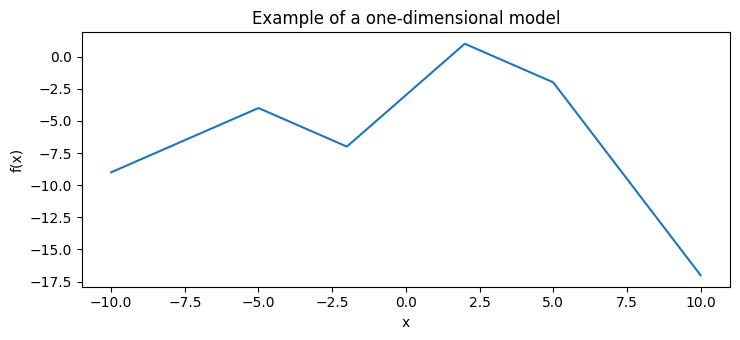
\includegraphics[width=14cm]{ex_3_1.png}
\end{center}
\caption{A plot produced using the exact model described in section \ref{piece:1d}. The plot was produced by evaluating the network on a set of 1000 points evenly spaced between the limits, as is commonly done so in programming to produce a line plot of a function.}
\end{figure}

Figure \ref{piece:ex_3_1} shows an example of the plot produced by the exact model with the values
\begin{align*}
    \left(a_1, a_2, a_3, a_4\right) &= \left(-5, -2, 2, 5\right) \\
    \left(m_0, m_1, m_2, m_3, m_4\right) &= \left(3, -1, 2, -1, -3\right) \\
    c &= 1.
\end{align*}
This is the same function that is used as the basis for training the approximate model.
\end{exa}

\begin{exa}
The function \verb|make_nd_model(a=,m=,c=)| builds a $d$-dimensional model from two lists and a constant. Each of the two lists are separated into $d$ lists representing the locations of the corners and the slopes in each dimension.

\begin{figure}[H]\label{piece:ex_3_2}
\begin{center}
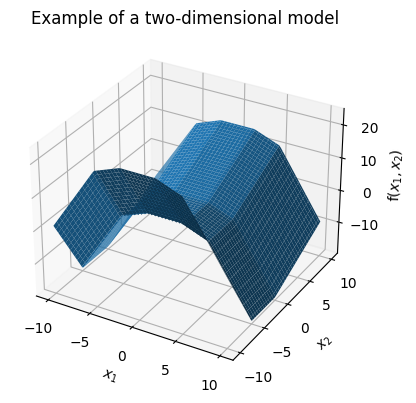
\includegraphics[width=12cm]{ex_3_2.png}
\end{center}
\caption{A plot produced using the exact model described in section \ref{piece:nd}. In this case, $d=2$. The technique again evaluated the network at each point, with the grid formed by crossing two sets of 1000 points between the limits for each axis.}
\end{figure}

Figure \ref{piece:ex_3_2} shows an example of a plot produced by the exact model with the values
\begin{align*}
    \left(a_{1,1}, a_{1,2}, a_{1,3}, a_{1,4}\right) &= \left(-5, -2, 2, 5\right) \\
    \left(a_{2,1}, a_{2,2}, a_{2,3}\right) &= \left(-5, 0, -5\right) \\
    \left(m_{1,0}, m_{1,1}, m_{1,2}, m_{1,3}, m_{1,4}\right) &= \left(4, 1, 0, -1, -4\right) \\
    \left(m_{2,0}, m_{2,1}, m_{2,2}, m_{2,3}\right) &= \left(4, 1, 0, -1\right) \\
    c &= 1.
\end{align*}
\end{exa}

\begin{exa}
The function \verb|make_approx_model(N=,r=)| initializes an approximate 1-D model using an existing exact model, and a learning rate. In this example we use the values from section \ref{piece:train} to create the exact model. It was found that a suitable value for the learning rate was 0.05.

The function \verb|train_approx_model(M=,N=,samples=,epochs=)| was used to train the approximate model using the initialized model, exact model, and values for the number of samples to generate in the training data and the maximum number of epochs to train for.

It was found that the model was able to replicate the function $f$ to various degrees of accuracy over different runs. Figure \ref{piece:ex_3_3} shows a collection of plots produced by the trained approximate model versus the given exact model.

\begin{figure}[H]\label{piece:ex_3_3}
\begin{center}
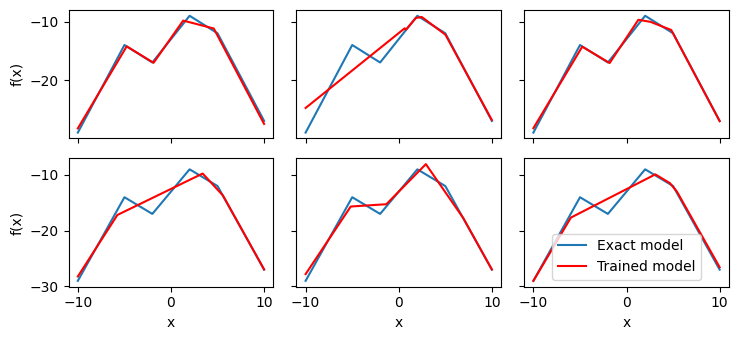
\includegraphics[width=14cm]{ex_3_3.png}
\end{center}
\caption{A collection of models trained as described in section \ref{piece:train}. We can see that some of them are identical, suggesting the same local minimum was reached during training.}
\end{figure}

Examining the weights of the trained models, it can be seen that where it is able to match the exact model, the trained model replicated the same weights up to multiplication and division by constants that cancel out between layers to arrive at the same result. This was only true for the intervals where a match was achieved. In some cases it can be seen that the model missed some of the corners and replaced multiple intervals with a single slope. When this happened, there were weights that were set to close to 0 across the layers, which caused corner points to disappear from the resulting plots.
\end{exa}

\section{Discussion}

\subsection{Exact models}

For the generalization we applied in this chapter, it was required that we divided the domain into (hyper-)rectangles so that we could write $f$ in the form of equation \ref{piece:eq2}. We could specify other continuous functions such as $f\left(x, y\right) := \left(x + y\right)_+$. This function can clearly be computed by a neural network with just one dense layer with a ReLU activation function, and could be considered to be piece-wise linear as the slopes are constant on two regions separated by the boundary along $y = -x$. In this case, we could still use equation \ref{piece:eq2} by inserting a dense layer to rotate the input 45 degrees clockwise from $\left(x, y\right)$ to $\left(\frac{\sqrt{2}\left(x+y\right)}{2}, \frac{\sqrt{2}\left(y-x\right)}{2}\right)$, and then evaluating $f\left(x,y\right)$ as
\begin{align*}
    f\left(x,y\right) = \left(\sqrt{2}\left(\frac{\sqrt{2}\left(x+y\right)}{2}\right) + 0 \left(\frac{\sqrt{2}\left(y-x\right)}{2}\right)\right)_+.
\end{align*}

It seems that we would be able to use this trick in any case where the domain is divided into (hyper-)rectangles with some linear transformation applied.

Another case of interest to consider would be dividing $\mathbb{R}^2$ into triangles, as this is a technique that is used to draw surfaces in computer graphics. It seems unlikely that the strategy we have used would work in this case, as the three boundaries of a triangle would mean that at least one of them is dependent on both variables whatever linear transformation is applied.

\subsection{Approximate models}

The aim of the training experiment was to see how well a model with the same layer architecture could replicate the exact model weights and biases. Visually it was clear that in some cases, the model was exactly or nearly-exactly matching the exact model. As the weights also matched the exact model in these cases, we were satisfied that the exact structure could be found through training.

As this result was confirmed with little effort put into optimizing the training, it could be possible that there were factors that we did not consider that would have improved the reliability of the training in order to match the exact model more often, such as adding a learning rate schedule or modifying the batch size. It appears that the random initialization may have caused the model to converge to local minima in some cases; further experimentation would be needed to identify these and determine whether they could be avoided in favour of the global minimum (exact match).

Optimization of the training process may also have been more relevant if this experiment was continued to 2- or 3-dimensional models to see if increasing the number of parameters prevented the model from replicating the exact structure.

\chapter{Searching for "zero" and "one"}

\section{Introduction}

This chapter will consider the task of searching for particular words in a string of text. A typical way to process text using neural networks is to use a word tokenizer, where each word is assigned an integer $w$ from 1 to $W$, where $W$ is the total size of the \textit{vocabulary} we have used during training. This integer is then translated into a \textit{one-hot encoded} vector, where the vector is a zero vector of length $W$, apart from the $w$-th entry which is set to 1. Applying a word tokenizer to the input would make searching for particular words in a given text string a trivial task, so the aim of the models implemented in this chapter is to take the input one character at a time.

In general, the neural networks in this chapter will be set up to take a string of one-hot encoded inputs $\left\{\pmb{x}_t\right\}_{t=1}^T$, and produce a series of one-hot encoded outputs $\left\{\pmb{y}_t\right\}_{t=1}^T$, corresponding to the completion of a detected word at input $\pmb{x}_t$.

Let $o_m: \left\{1, \dots, m\right\} \rightarrow \left\{0, 1\right\}^m$ denote one-hot encoding, where the one-hot encoded vector $o_m\left(n\right)$ in $\left\{0,1\right\}^m$ is 1 in the $n$-th position and 0 everywhere else.

\section{Methods}

The methods described in this section are implemented in the file \url{https://github.com/HectorLeitch/mas6041/blob/main/code/zeroone.py}.

\subsection{Small input model}\label{zeroone:small}

We will start by building a network to detect two words: "zero" and "one". For simplicity, we will assume that all punctuation has been removed from the text. To reduce the size of the one-hot encoded inputs in order to help build an initial model, each character $w_t$ will be mapped to $\pmb{x}_t$ according to the following:
\begin{align}
    \mathbf{x}\left(w\right) =
    \begin{cases}
        o_7\left(1\right) & w = \text{" " (space)} \\
        o_7\left(2\right) & w = \text{"z"} \\
        o_7\left(3\right) & w = \text{"e"} \\
        o_7\left(4\right) & w = \text{"r"} \\
        o_7\left(5\right) & w = \text{"o"} \\
        o_7\left(6\right) & w = \text{"n"} \\
        o_7\left(7\right) & \text{otherwise}
    \end{cases}
\end{align}
This reduction in size allows us to create the weights in the first layer by hand without dealing with the large weights matrix required to process one-hot encoded inputs of size 128. The columns can then be translated into the full model.

The first layer $\mathcal{L}^{\left[1\right]}$ of the neural network will be a recurrent layer. This layer will take the individual inputs, and cycle through a finite number of states in order to detect the words. The output will be a vector of length 10, constructed as follows:
\begin{align}
    \mathcal{L}^{\left[1\right]}\left(\pmb{x}_t\right)
    \begin{pmatrix}
        \pmb{p}_t \in \left\{0,1\right\}^7 \\
        \pmb{q}_t \in \left\{0,1\right\}^2 \\
        r_t \in \left\{0,1\right\}
    \end{pmatrix}
\end{align}
where
\begin{itemize}
    \item $\mathbf{p}_t$ is a one-hot encoding using $o_7$, and represents the possible sequences that are detected within the words "zero" and "one": "z", "ze", "zer", "zero", "o", "on", "one". If nothing is detected, it can also be $\mathbf{0}$.
    \item $\mathbf{q}_t$ is a one-hot encoding using $o_2$ which represents whether a "zero" or "one" has been detected. If neither is detected, it can also be $\mathbf{0}$.
    \item $r_t$ is a "blocking" indicator, which stops $\mathbf{p}_t$ from moving into a one-hot encoding if $w_{t-1}$ is not a space. This prevents the detection of words within other words, such as "one" within "gone".
\end{itemize}

The weights matrix applied to the input $\pmb{x}_t$ is
\begin{align}
\mathbf{W}_1 =
\begin{pmatrix}
 0 & 1 & 0 & 0 & 0 & 0 & 0\\
 0 & 0 & 1 & 0 & 0 & 0 & 0\\
 0 & 0 & 0 & 1 & 0 & 0 & 0\\
 0 & 0 & 0 & 0 & 1 & 0 & 0\\
 0 & 0 & 0 & 0 & 1 & 0 & 0\\
 0 & 0 & 0 & 0 & 0 & 1 & 0\\
 0 & 0 & 1 & 0 & 0 & 0 & 0\\
 1 & 0 & 0 & 0 & 0 & 0 & 0\\
 1 & 0 & 0 & 0 & 0 & 0 & 0\\
-1 & 1 & 1 & 1 & 1 & 1 & 1
\end{pmatrix}.
\end{align}
In $\mathbf{W}_1$, each column corresponds to a value in the input and each row corresponds to a value in the resulting output state. The entries determine adjustments to each value of the output state depending on which input is received. The first column indicates that when $w_t$ is a space, both one-hot states of $\pmb{q}_t$ are possible (rows 8 and 9), and furthermore that the blocking indicator $r_t$ should be reduced from 1 to 0 as a new sequence may start following the space. The next five columns correspond to possible states of $\pmb{p}_t$ where letter sequences have been detected, and $r_t$ is set to 1 to prevent a new sequence starting. The final column resets $\pmb{p}_t$ if $w_t$ is any other character, and also sets $r_t$ to 1.

The weights matrix applied to the previous state $\mathcal{L}^{\left[1\right]}\left(\pmb{x}_{t-1}\right)$ is
\begin{align}
\mathbf{U}_1 =
\begin{pmatrix}
0 & 0 &  0 & 0 & 0 & 0 & 0 & 0 & 0 & -1\\
1 & 0 &  0 & 0 & 0 & 0 & 0 & 0 & 0 &  0\\
0 & 1 &  0 & 0 & 0 & 0 & 0 & 0 & 0 &  0\\
0 & 0 &  1 & 0 & 0 & 0 & 0 & 0 & 0 &  0\\
0 & 0 & -1 & 0 & 0 & 0 & 0 & 0 & 0 & -1\\
0 & 0 &  0 & 0 & 1 & 0 & 0 & 0 & 0 &  0\\
0 & 0 &  0 & 0 & 0 & 1 & 0 & 0 & 0 &  0\\
0 & 0 &  0 & 1 & 0 & 0 & 0 & 0 & 0 &  0\\
0 & 0 &  0 & 0 & 0 & 0 & 1 & 0 & 0 &  0\\
0 & 0 &  0 & 0 & 0 & 0 & 0 & 0 & 0 &  0
\end{pmatrix}.
\end{align}
In $\mathbf{U}_1$, the rows again correspond a value in the resulting output state, but the entries determine adjustments to each value of the output state depending on which previous output state is received. The columns correspond to a value in the previous output state.
\begin{itemize}
    \item The first column indicates that if the previous state contains $\pmb{p}_{t-1} = o_7\left(1\right)$ i.e. "z" detected, then $\pmb{p}_t$ may equal $o_7\left(1\right)$ i.e. "ze" detected. The second, fifth, and sixth columns are similar.
    \item The third column indicates that if the previous state contains $\pmb{p}_{t-1} = o_7\left(3\right)$ i.e. "zer" detected, then $\pmb{p}_t$ may equal $o_7\left(4\right)$  i.e. "zero" detected, and also should not equal $o_7\left(5\right)$ i.e. "o" detected.
    \item The fourth column indicates that if the previous state contains $\pmb{p}_{t-1} = o_7\left(4\right)$ i.e. "zero" detected, then $\pmb{q}_t$ may equal $o_2\left(1\right)$ i.e. output "zero". The seventh column is similar.
    \item The tenth column indicates that if $r_{t-1}$ is 1, then $\pmb{p}_t$ should not equal $o_7\left(1\right)$ i.e. "z" detected, or $o_7\left(5\right)$ i.e. "o" detected. This "blocks" the next state from starting the detection of a new word.
\end{itemize}

The bias 
\begin{align}
\pmb{b}_1^T =
\begin{pmatrix}
0 & -1 & -1 & -1 & 0 & -1 & -1 & -1 & -1 & 0
\end{pmatrix}
\end{align}
adjusts the entries where necessary so that, combined with a ReLU activation on the layer, the values are either 1 or 0.

We now observe that $\pmb{q}_t$ constitutes a suitable output for the network as a whole. We can either take the output from the first layer and discard the rest, or attach a dense layer $\mathcal{L}^{\left[2\right]}$ to the recurrent layer output with
\begin{align}
\mathcal{L}^{\left[2\right]}\left(\pmb{x}_t\right) =
\begin{pmatrix}
    0 & 0 & 0 & 0 & 0 & 0 & 0 & 1 & 0 & 0 \\
    0 & 0 & 0 & 0 & 0 & 0 & 0 & 0 & 1 & 0
\end{pmatrix}
\mathcal{L}^{\left[1\right]}\left(\pmb{x}_t\right),
\end{align}
where the bias is $\mathbf{0}$ and the activation function is the linear activation function.

\subsection{Full model}\label{zeroone:full}

We can expand this model to a "full" model, where each character has a value assigned using the Python \verb|ord()| function. This translates characters into their Unicode values, which we will assume are limited to ASCII values of 0 to 127.

The only change required in the model is to $\mathbf{W}_1$, which will have 128 columns. We simply copy the columns specified in the previous model to handle each character appropriately:
\begin{itemize}
    \item The ASCII value for "Z" and "z" are 90 and 122 respectively. Therefore, column 91 and 123 of $\mathbf{W}_1$ are set to $\begin{pmatrix}
        1 & 0 & 0 & 0 & 0 & 0 & 0 & 0 & 0 & 1
    \end{pmatrix}^T$.
    \item The ASCII value for "E" and "e" are 69 and 101 respectively. Therefore, column 70 and 102 of $\mathbf{W}_1$ are set to $\begin{pmatrix}
        0 & 1 & 0 & 0 & 0 & 0 & 1 & 0 & 0 & 1
    \end{pmatrix}^T$.
    \item The ASCII value for "R" and "r" are 82 and 114 respectively. Therefore, column 83 and 115 of $\mathbf{W}_1$ are set to $\begin{pmatrix}
        0 & 0 & 1 & 0 & 0 & 0 & 0 & 0 & 0 & 1
    \end{pmatrix}^T$.
    \item The ASCII value for "O" and "o" are 79 and 111 respectively. Therefore, column 80 and 112 of $\mathbf{W}_1$ are set to $\begin{pmatrix}
        0 & 0 & 0 & 1 & 1 & 0 & 0 & 0 & 0 & 1
    \end{pmatrix}^T$.
    \item The ASCII value for "N" and "n" are 78 and 110 respectively. Therefore, column 79 and 111 of $\mathbf{W}_1$ are set to $\begin{pmatrix}
        0 & 0 & 0 & 0 & 0 & 1 & 0 & 0 & 0 & 1
    \end{pmatrix}^T$.
    \item The ASCII values for other alpha-numeric characters are 48 to 57 for numbers 0 to 9, 65 to 90 for uppercase letters, and 97 to 122 for lowercase letters. Therefore, columns 49 to 58, 66 to 91, and 98 to 123 (excluding those assigned above) of $\mathbf{W}_1$ are set to $\begin{pmatrix}
        0 & 0 & 0 & 0 & 0 & 0 & 0 & 0 & 0 & 1
    \end{pmatrix}^T$.
    \item The remaining ASCII values include space (32) and other punctuation. Therefore, the remaining columns of $\mathbf{W}_1$ are set to \\ $\begin{pmatrix}
        0 & 0 & 0 & 0 & 0 & 0 & 0 & 1 & 1 & -1
    \end{pmatrix}^T$.
\end{itemize}

As we are still only detecting "zero" and "one" with this model, we do not need any more states. The other parts are therefore unchanged.

\subsection{Input padding}

In the models above, we have not added anything to the end of the input but we can see that a word is only detected when it is followed by a space (or other punctuation). In both models, we therefore "pad" the input with a space at the end. This ensures that the strings "zero" and "one" given on their own are detected.


\section{Results}

The models described above are demonstrated in the Jupyter notebook \url{https://github.com/HectorLeitch/mas6041/blob/main/try_zeroone.ipynb}. The notebook is split into examples to demonstrate the code, which are described in the following paragraphs.

\begin{exa}
The function \verb|make_rnn_model()| builds the model described in section \ref{zeroone:small}. The input is a text string that is then padded and converted into a sequence of one-hot encoded vectors, each of length 7.

The output is a sequence of vectors, each of length 2. A 1 in the first entry corresponds to detecting "zero" and a 1 in the second entry corresponds to detecting "one". If neither are detected, both entries will be 0.
\end{exa}

\begin{exa}
The function \verb|make_full_rnn_model()| builds the model described in section \ref{zeroone:full}. The input is a text string that is then padded and converted into a sequence of one-hot encoded vectors, each of length 128. The output is the same as the example above.
\end{exa}

\section{Discussion}

\subsection{Finite state machine}

The neural networks in this chapter were designed to create an underlying finite state machine, where the state is captured in $\pmb{p}_t$ and a "base" state is represented by $\mathbf{0}$. The addition of $\pmb{q}_t$ and $r_t$ was an intuitive way to develop the handling of the rule where "zero" and "one" are only counted if they appear as isolated words.

\subsection{Possible extension}

Given that the underlying model is a finite state machine, we could add any finite number of words to our list of words to detect. For example, if we wanted to detect the words for all digits from "zero" to "nine", we could build a network where $\pmb{p}_t$ has states for "z", "ze", "zer", "zero", "o", "on", "one", "t", etc., up to "n", "ni", "nin", and "nine", and $\pmb{q}_t \in \left\{0,1\right\}^{10}$ has an output for each digit.

In the first model, the third and fifth column of $\mathbf{W}_1$, and the third column of $\mathbf{U}_1$ give the strategies required to handle letters that are shared between the words. For example, the column in $\mathbf{U}_1$ corresponding to "seven" detected should have a -1 in the row corresponding to "n" detected to prevent the next state moving to "ni".



\chapter{Letter and word detection}

\section{Introduction}\label{letters:intro}.

This chapter will introduce convolutional neural networks (CNNs) for processing images. We will build a simple neural network to find letters in an image, and with some additional assumptions extend it to a neural network that can identify words.

The assumptions we will make throughout this chapter are that an input image $\mathbf{X}$ is a matrix with $w$ columns and $h$ rows, and entries in $\left\{0,1\right\}$ where 0 represents a white pixel and 1 represents a black pixel. Furthermore, the input $\mathbf{X}$ will contain letters from the set $\left\{I, Y, J, C, O, L, H, T, U, X\right\}$, written in uppercase. These letters can be represented by matrices in $M_{3,3}\left\{0,1\right\}$. Denote the matrix representing the letter $a \in \left\{I, Y, J, C, O, L, H, T, U, X\right\}$ as $A_a \in M_{3,3}\left\{0,1\right\}$.

After building the convolutional layer required to detect these letters, we will attach further layers to build models that can keep track of counts of each letter, and recognise words from a given list containing words using only the letters in $\left\{I, Y, J, C, O, L, H, T, U, X\right\}$.

Explicitly, the $3 \times 3$ matrices are as follows:
\begin{center}
\begin{tabular}{c c}
    $\mathbf{A}_I =
    \begin{pmatrix}
        0 & 1 & 0 \\
        0 & 1 & 0 \\
        0 & 1 & 0
    \end{pmatrix}$ &
    $\mathbf{A}_Y =
    \begin{pmatrix}
        1 & 0 & 1 \\
        0 & 1 & 0 \\
        0 & 1 & 0
    \end{pmatrix}$ \\
    $\mathbf{A}_J =
    \begin{pmatrix}
        0 & 0 & 1 \\
        0 & 0 & 1 \\
        1 & 1 & 1
    \end{pmatrix}$ &
    $\mathbf{A}_C =
    \begin{pmatrix}
        1 & 1 & 1 \\
        1 & 0 & 0 \\
        1 & 1 & 1
    \end{pmatrix}$ \\
    $\mathbf{A}_O =
    \begin{pmatrix}
        1 & 1 & 1 \\
        1 & 0 & 1 \\
        1 & 1 & 1
    \end{pmatrix}$ &
    $\mathbf{A}_L =
    \begin{pmatrix}
        1 & 0 & 0 \\
        1 & 0 & 0 \\
        1 & 1 & 1
    \end{pmatrix}$
\end{tabular}
\begin{tabular}{c c}
    $\mathbf{A}_H =
    \begin{pmatrix}
        1 & 0 & 1 \\
        1 & 1 & 1 \\
        1 & 0 & 1
    \end{pmatrix}$ &
    $\mathbf{A}_T =
    \begin{pmatrix}
        1 & 1 & 1 \\
        0 & 1 & 0 \\
        0 & 1 & 0
    \end{pmatrix}$ \\
    $\mathbf{A}_U =
    \begin{pmatrix}
        1 & 0 & 1 \\
        1 & 0 & 1 \\
        1 & 1 & 1
    \end{pmatrix}$ &
    $\mathbf{A}_X =
    \begin{pmatrix}
        1 & 0 & 1 \\
        0 & 1 & 0 \\
        1 & 0 & 1
    \end{pmatrix}$
\end{tabular}
\end{center}

\section{Methods}

The methods described in this section are implemented in the file \url{https://github.com/HectorLeitch/mas6041/blob/main/code/letters.py}.

\subsection{Letter recognition}\label{letters:letter}

We will start by building convolutional kernels to recognise each letter, in a neural network with just a single convolutional layer. For this step we will restrict an input $\mathbf{X}$ to be $3 \times 3$, so that with a $3 \times 3$ kernel a single output value is given.

For a given $a \in \left\{I, Y, J, C, O, L, H, T, U, X\right\}$, let $S_a = \left\{\left(i, j\right) | \left[\mathbf{A}_a\right]_{i,j} = 1\right\}$. Then, for any input $\mathbf{X} \in M_{3,3}\left\{0,1\right\}$, we have
\begin{align}\label{letters:eq0}
I\left(\mathbf{X} = \mathbf{A}_a\right) = \left(1 + \sum_{i, j \in S_a} \left[\mathbf{X}\right]_{i,j} - \sum_{i, j \notin S_a} \left[\mathbf{X}\right]_{i,j} - \sum_{i,j} \left[\mathbf{A}_a\right]_{i,j}\right)_+.
\end{align}

It follows that we can create a kernel $\mathbf{W}_a$ by setting $\left[\mathbf{W}_a\right]_{i,j}$ to 1 for $\left(i,j\right) \in S_a$ and -1 for $\left(i,j\right) \notin S_a$, i.e.
\begin{align*}
\mathbf{W}_a = 2\mathbf{A}_a - \mathbf{1}_{3,3}.
\end{align*}
We combine this with a bias term $\mathbf{b}_a = 1 - \sum_{i,j} \left[\mathbf{A}_a\right]_{i,j}$, and the RelU activation function so that the output values are only 0 or 1.

To create the first neural network, we combine the kernels $\mathbf{W}_a$ and biases $\pmb{b}_a$ for each $a \in \left\{I, Y, J, C, O, L, H, T, U, X\right\}$, resulting in a layer $\mathcal{L}^{\left[1\right]}$ with 10 channels.

\subsection{Expanding the grid}\label{letters:expand}

The previous model was restricted to producing a single output in $\left\{0,1\right\}$ for each channel, in the sense that the convolution kernels did not move across the spatial dimensions of the input $\mathbf{X}$, as we restricted the size of the input to match the size of the kernels. We will now consider inputs $\mathbf{X} \in M_{h,w}\left\{0,1\right\}$, where $w,h > 3$.

For this model, some further assumptions will be made about $\mathbf{X}$.
\begin{itemize}
    \item $\mathbf{X}$ may contain multiple sub-matrices $\mathbf{A}_a$, or none at all. And the sub-matrix for each letter $a$ may appear more than once.
    \item The letters are all written from left to right on a single "line", although the vertical positions may be anywhere such that they fit within the height $h$.
    \item Each letter occupies the whole of its $3 \times 3$ sub-matrix, and the sub-matrices of more than one letter cannot overlap.
\end{itemize}

The first layer of the model is a convolutional layer with 10 channels, where the weights, biases, and activation is from the first model. Now the kernels move across the dimensions of the image $\mathbf{X}$, the result for each channel will be a feature map of size $\left(h - 2\right) \times \left(w - 2\right)$.

As we have assumed that the letters will not overlap, we can then pass the output $\mathcal{L}^{\left[1\right]}\left(\mathbf{X}\right)$ to a max pooling layer. The additional assumptions we have made about $\mathbf{X}$ mean that we know each letter can only be present once within each vertical $h \times 3$ slice, so we can set this to be the pool size. We apply zero padding to $\mathcal{L}^{\left[1\right]}\left(\mathbf{X}\right)$, so the output $\mathcal{L}^{\left[2\right]}\left(\mathbf{X}\right)$ will be of size $1 \times \lfloor w/3 \rfloor$ in each channel. Therefore, as the pool moves across $\mathcal{L}^{\left[1\right]}\left(\mathbf{X}\right)$, the corresponding output will be 1 each time a letter is detected within each corresponding channel.

This output is sufficient to show detection of each letter, but for the following models we will consider reshaping the output into a sequence of $w_g = \lfloor w/3 \rfloor$ vectors, where each vector is in $\left\{0,1\right\}$ and is either $\mathbf{0}$ for no letter detected, or a one-hot encoding of a detected letter. For example, the sequence
\begin{align*}
    &\begin{pmatrix}
        0 & 0 & 0 & 1 & 0 & 0 & 0 & 0 & 0 & 0
    \end{pmatrix}^T, \\
    &\begin{pmatrix}
        1 & 0 & 0 & 0 & 0 & 0 & 0 & 0 & 0 & 0
    \end{pmatrix}^T, \\
    &\begin{pmatrix}
        0 & 0 & 0 & 0 & 0 & 0 & 0 & 1 & 0 & 0
    \end{pmatrix}^T, \\
    &\begin{pmatrix}
        0 & 1 & 0 & 0 & 0 & 0 & 0 & 0 & 0 & 0
    \end{pmatrix}^T
\end{align*}
represents the detection of the letters $\left(\text{"C", "I", "T", "Y"}\right)$.

\subsection{Counting occurrences}\label{letters:count}

Suppose now that we wish to count the number of occurrences of each letter within the input grid. This can be done by attaching a dense layer $\mathcal{L}^{\left[3\right]}$ with input $\mathcal{L}^{\left[2\right]}\left(\mathbf{X}\right)$ from the model above.

The input to this layer $\mathcal{L}^{\left[2\right]}\left(\mathbf{X}\right)$ should be reshaped so that it has 10 columns, one for each letter, and $w_g$ rows. It is then passed to the dense layer as a single input in $\left\{0,1\right\}^{w_g \time 10}$. We can then extract the sums of each of the letters by simply multiplying this input with the vector of ones $\mathbf{1}_{10}$, adding no bias or activation function.

\subsection{Recognising words}\label{letters:words}

To recognise words, we wish to take the output from $\mathcal{L}^{\left[2\right]}\left(\mathbf{X}\right)$ and convert this into a unique integer sequence to represent a detected word. For example, the detection of the word $\left(\text{"C", "I", "T", "Y"}\right)$ would be recognised from the sequence
$\begin{pmatrix}
    4 & 1 & 8 & 2 & 0 & \dots & 0
\end{pmatrix} \in \left\{0, \dots, 10\right\}^{w_g}$.

The problem to solve is that we may encounter gaps in the letters and so after converting the one-hot outputs to integers, they will not necessarily be in the left-most positions and there may be zeros between them. We therefore need a way to process the sequence to move the non-zero entries to the start whilst retaining their order.

We will go through two different ways that this can be achieved.

The first model takes the following steps:
\begin{itemize}
    \item Convert each zero or one-hot vector into an integer $x_t \in \left\{0, \dots, 10\right\}$.
    \item Create an indicator $I\left(x_t > 0\right)$ for $t=1, \dots, w_g$.
    \item Create a running counter $s_t$ that starts at 0 and increments when $x_t > 0$. This indicates the intended final position for each non-zero $x_t$.
    \item For each $i \in \left\{1, \dots, w_g\right\}$, create an indicator $I\left(s_t = i\right)$.
    \item Combine the indicators to create $I\left(x_t > 0 \text{ and } s_t = i\right)$ for $i \in \left\{1, \dots, w_g\right\}$.
    \item Build the final sequence by adding $x_t$ into position $i$ if $I\left(x_t > 0\right)$ and $I\left(s_t = i\right)$. We will see that the previous steps have been designed to allow this step to be done quite directly with a gated recurrent unit layer.
\end{itemize}

Following the max pooling layer $\mathcal{L}^{\left[2\right]}$, the conversion to an integer sequence can be done through a dense layer. Treating $\mathcal{L}^{\left[2\right]}\left(\mathbf{X}\right)$ as a $10 \times w_g$ matrix, we can multiply by weights $\mathbf{W}_3 =
\begin{pmatrix}
    1 & 2 & \dots & 10
\end{pmatrix}$, adding no bias or activation function, so the output is
\begin{align*}
\mathcal{L}^{\left[3\right]}\left(\mathbf{X}\right) =
\begin{pmatrix}
    1 & 2 & \dots & 10
\end{pmatrix}
\mathcal{L}^{\left[2\right]}\left(\mathbf{X}\right).
\end{align*}

This converts each one-hot encoded column in $\mathcal{L}^{\left[2\right]}\left(\mathbf{X}\right)$ into an integer and the value is given by the position of the 1 in each column. In the case that no letters are detected, the value is set to 0. We may now consider this as a vector $\mathcal{L}^{\left[3\right]}\left(\mathbf{X}\right) \in \left\{0, \dots, 10\right\}^{w_g}$, or a sequence $\mathcal{L}^{\left[3\right]}\left(\mathbf{X}\right) = \left\{x_t\right\}_{t=1}^{w_g}$ where $x_t \in \left\{0, \dots, 10\right\} \forall t$.

We now wish to produce another sequence $\left\{I\left(x_t > 0\right)\right\}_{t=1}^{w_g}$. Observe that for $x, n \in \mathbb{Z}$,
\begin{align}\label{letters:eq1}
I\left(x > n\right) = \left(x - n\right)_+ - \left(x - n - 1\right)_+.
\end{align}
If we consider the output $\mathcal{L}^{\left[3\right]}\left(\mathbf{X}\right) = \left\{x_t\right\}_{t=1}^{w_g}$ as a sequence, we can create the corresponding sequence of indicators in two dense layers $\mathcal{L}^{\left[4\right]}$ and $\mathcal{L}^{\left[5\right]}$, where
\begin{align*}
\mathcal{L}^{\left[4\right]}\left(x_t\right) = \left(
\begin{pmatrix}
    1 \\
    1
\end{pmatrix}
x_t +
\begin{pmatrix}
    0 \\
    -1
\end{pmatrix}\right)_+,
\end{align*}
and
\begin{align*}
\mathcal{L}^{\left[5\right]}\left(x_t\right) =
\begin{pmatrix}
    1 \\
    -1
\end{pmatrix}
\mathcal{L}^{\left[4\right]}\left(x_t\right).
\end{align*}

We now wish to create the sequence $\left\{s_t\right\}_{t=1}^{w_g}$. This will utilise a simple gated recurrent unit (GRU) layer, $\mathcal{L}^{\left[6\right]}$, using the previous sequence $\left\{I\left(x_t > 0\right)\right\}_{t=1}^{w_g}$ as input. Starting with $y_0 = 0$, at time $t$ the GRU will propose a new state $\hat{y}_t = y_{t-1} + 1$ and then set $z_t = 1 - I\left(x_t > 0\right)$. Therefore,
\begin{align*}
x_t > 0 &\implies z_t = 0 \\
&\implies y_t = \hat{y}_t = y_{t-1} + 1,
\end{align*}
and conversely
\begin{align*}
x_t = 0 &\implies z_t = 1 \\
&\implies y_t = y_{t-1}.
\end{align*}

Explicitly, this means in the GRU layer:
\begin{itemize}
    \item $\mathbf{W}^{\left[6\right]}_r = \mathbf{U}^{\left[6\right]}_r = \pmb{b}^{\left[6\right]}_r = 0 \implies r_t = 0 \forall t$
    \item $\mathbf{W}^{\left[6\right]}_z = -1, \mathbf{U}^{\left[6\right]}_z = 0, \pmb{b}^{\left[6\right]}_z = 1 \implies z_t = 1 - I\left(x_t > 0\right)$.
    \item $\mathbf{W}^{\left[6\right]}_y = 0, \mathbf{U}^{\left[6\right]}_y = 1, \pmb{b}^{\left[6\right]}_y = 1 \implies \hat{y}_t = y_{t-1} + 1$.
\end{itemize}

The output $\mathcal{L}^{\left[6\right]}\left(x_t\right) = s_t$ is then set to $y_t$.

We now create a sequence of vectors $\left\{\pmb{p}_t\right\}_{t=1}^{w_g}$, where each $\pmb{p}_t$ is $I\left(s_t = i\right)$ for $i = 1, \dots, w_g$. Alternatively, we could view $\pmb{p}_t$ as the one-hot encoding $o_{w_g}\left(s_t\right)$. We can re-use the structure we used to create $I\left(x_t > 0\right)$, observing that for $x,n \in \mathbb{Z}$,
\begin{align*}
I\left(x = n\right) = \left(1 + x - n\right)_+ - 2\left(x - n\right)_+ + \left(x - n - 1\right)_+.
\end{align*}

Therefore, we add dense layers $\mathcal{L}^{\left[7\right]}$ and $\mathcal{L}^{\left[8\right]}$, where
\begin{align*}
\mathcal{L}^{\left[7\right]}\left(s_t\right) = \left(
\begin{pmatrix}
    1 \\
    1 \\
    1 \\
    \dots \\
    1 \\
    1 \\
    1
\end{pmatrix}
s_t +
\begin{pmatrix}
    1 \\
    0 \\
    -1 \\
    \dots \\
    w_g + 1 \\
    w_g \\
    w_g - 1
\end{pmatrix}\right)_+,
\end{align*}
and
\begin{align*}
\mathcal{L}^{\left[8\right]}\left(s_t\right) =
\begin{pmatrix}
    1 & -2 & 1 & 0 & 0 & 0 & \dots & 0 & 0 & 0 \\
    0 & 0 & 0 & 1 & -2 & 1 & \dots & 0 & 0 & 0 \\
    \dots & \dots & \dots & \dots & \dots & \dots & \dots & \dots & \dots & \dots \\
    0 & 0 & 0 & 0 & 0 & 0 &\dots & 1 & -2 & 1
\end{pmatrix}
\mathcal{L}^{\left[7\right]}\left(s_t\right).
\end{align*}

The last part before the GRU layer is combining the indicators we have produced so far into a sequence of vectors $\left\{\pmb{q}_t\right\}_{t=1}^{w_g}$, where each $\pmb{q}_t$ is $I\left(x_t > 0 \text{ and } s_t = i\right)$ for $i = 1, \dots, w_g$. This can be done in a single dense layer $\mathcal{L}^{\left[9\right]}$ where the input is the concatenation $\left(\mathcal{L}^{\left[5\right]}\left(x_t\right), \mathcal{L}^{\left[8\right]}\left(s_t\right)\right)$, which is a vector of length $w_g + 1$. The calculation for $\mathcal{L}^{\left[9\right]}$ is
\begin{align*}
\mathcal{L}^{\left[9\right]}\left(\mathcal{L}^{\left[5\right]}\left(x_t\right), \mathcal{L}^{\left[8\right]}\left(s_t\right)\right) = \left(
\begin{pmatrix}
    1 & 1 & 0 & \dots & 0 \\
    1 & 0 & 1 & \dots & 0 \\
    \dots & 0 & 0 & \ddots & \dots \\
    1 & 0 & 0 & \dots & 1
\end{pmatrix}
\begin{pmatrix}
    \mathcal{L}^{\left[5\right]}\left(x_t\right) \\
    \mathcal{L}^{\left[8\right]}\left(s_t\right)
\end{pmatrix}
- \mathbf{1}_{w_g}\right)_+,
\end{align*}
where the weights matrix is of size $w_g \times \left(w_g + 1\right)$.

The final layer yielding the desired sequence is a GRU layer, which takes $\left(x_t, \pmb{q}_t\right)$ as input. The components are set as follows:
\begin{align*}
\pmb{r}_t &= \mathbf{1}_{w_g}, \\
\pmb{z}_t &= \left(\mathbf{1}_{w_g} - \pmb{q}_t\right)_+, \\
\hat{\pmb{y}}_y &= \mathbf{1}_{w_g} x_t.
\end{align*}
which implies
\begin{align*}
\left[\pmb{y}_t\right]_i =
\begin{cases}
    \left[\pmb{y}_{t-1}\right]_i & x_t = 0 \text{ or } s_t \neq i \\
    x_t & x_t > 0 \text{ and } s_t = i.
\end{cases}
\end{align*}
So $\pmb{y}_0$ is initialised as $\mathbf{0}$, and the $i$-th entry is updated with the $i$-th non-zero value in $\left\{x_t\right\}_{t=1}^{w_g}$. We then take only the final state $\pmb{y}_{w_g}$ as the output of this layer, which yields the sequence with all non-zeros shifted to the start.

Explicitly, for the GRU layer $\mathcal{L}^{\left[10\right]}$, we have

\studentcomment{add weights here}

\subsection{Alternative shift method}\label{letters:alt}

The model in the previous section contains a lot of layers, spread between many separate stages. We now present an alternative architecture which slightly reduces the number of layers.

The aim is to reduce the number of layers required to take the indicator $I\left(x_t > 0\right)$ for $t=1, \dots, w_g$, and produce the sequence $\left\{\pmb{q}_t\right\}_{t=1}^{w_g}$ directly in one layer. This eliminates the need to build the running counter $s_t$ and then feed that into another two layers to produce indicators.

The modification replaces the layers $\mathcal{L}^{\left[6\right]}, \mathcal{L}^{\left[7\right]}$, and $\mathcal{L}^{\left[8\right]}$ with a single GRU layer $\mathcal{L}^{\left[6*\right]}$. We create a hidden state $\pmb{y}_t \in \left\{0, 1\right\}^{w_g+1}$, which we initialize as
\begin{align*}
\pmb{y}_0 =
\begin{pmatrix}
    1 & 0 & \dots & 0
\end{pmatrix}^T.
\end{align*}
The idea is to propose $\hat{\pmb{y}}_t$ to be the right-shifted $\pmb{y}_{t-1}$, and use the input $I\left(x_t > 0\right)$ to determine whether or not to update $\pmb{y}_t$. We can then drop the first element of $\pmb{y}_t$ to give us $\pmb{p}_t$, by adjusting the weights in the following layer to ignore the first entry of $\pmb{y}_t$.

Explicitly, we have:
\begin{align*}
&\begin{rcases}
    \mathbf{W}^{\left[6*\right]}_r = \mathbf{0}_{w_g+1} \\
    \mathbf{U}^{\left[6*\right]}_r = \mathbf{0}_{w_g+1 \times w_g+1} \\
    \pmb{b}^{\left[6*\right]}_r = \mathbf{1}_{w_g+1}
\end{rcases} \implies \pmb{r}_t = \mathbf{1}_{w_g+1} \forall t \\
\\
&\begin{rcases}
    \mathbf{W}^{\left[6*\right]}_z = -\mathbf{1}_{w_g+1} \\
    \mathbf{U}^{\left[6*\right]}_z = \mathbf{0}_{w_g+1 \times w_g+1} \\
    \pmb{b}^{\left[6*\right]}_z = \mathbf{1}_{w_g+1}
\end{rcases} \pmb{z}_t = \mathbf{1}_{w_g+1} - I\left(x_t > 0\right) \text{ (element-wise)} \\
\\
&\begin{rcases}
    \mathbf{W}^{\left[6*\right]}_y = \mathbf{0}_{w_g+1} \\
    \mathbf{U}^{\left[6*\right]}_y = \mathbf{R}_{w_g+1} \\
    \pmb{b}^{\left[6*\right]}_y = \mathbf{0}_{w_g+1}
\end{rcases} \implies \hat{\pmb{y}}_t = \mathbf{R} \pmb{y}_{t-1}
\end{align*}
where $\mathbf{R}_{w_g+1}$ is the "right-shift" matrix (although $\pmb{y}_t$ is a column vector in our notation)
\begin{align*}
\mathbf{R}_{w_g+1} =
\begin{pmatrix}
    0 & 1 & 0 & \dots & 0 \\
    0 & 0 & 1 & \dots & 0 \\
    \dots & \dots & \ddots & \ddots & 0 \\
    0 & \dots & \dots & 0 & 1
\end{pmatrix}.
\end{align*}

We now replace $\mathcal{L}^{\left[9\right]}$ with a slightly modified version $\mathcal{L}^{\left[9*\right]}$, to account for the extra input which we do not wish to use. For this layer we have
\begin{align*}
\mathcal{L}^{\left[9*\right]}\left(\mathcal{L}^{\left[5\right]}\left(x_t\right), \mathcal{L}^{\left[6*\right]}\left(x_t\right)\right) = \left(
\begin{pmatrix}
    1 & 0 & 1 & 0 & \dots & 0 \\
    1 & 0 & 0 & 1 & \dots & 0 \\
    \dots & 0 & 0 & 0 & \ddots & \dots \\
    1 & 0 & 0 & 0 & \dots & 1
\end{pmatrix}
\begin{pmatrix}
    \mathcal{L}^{\left[5\right]}\left(x_t\right) \\
    \mathcal{L}^{\left[6*\right]}\left(x_t\right)
\end{pmatrix}
- \mathbf{1}_{w_g}\right)_+.
\end{align*}
The output of $\mathcal{L}^{\left[9*\right]}$ and $\mathcal{L}^{\left[9\right]}$ will be identical so the final layer $\mathcal{L}^{\left[10\right]}$ is unchanged.

\section{Results}

The models described above are demonstrated in the Jupyter notebook \url{https://github.com/HectorLeitch/mas6041/blob/main/try_letters.ipynb}. The notebook is split into examples to demonstrate the code, which are described in the following paragraphs.

\begin{exa}
The function \verb|make_explicit_model()| builds a model to recognise letters given as a $3 \times 3$ image, as described in section \ref{letters:letter}.

We verify that it correctly identifies a single letter input, and furthermore rejects an input (i.e. does not claim to detect any letter) given a randomly generated input that does not happen to be a letter.

The function \verb|test_explicit_model()| verifies the model is working correctly on all possible $3 \times 3$ images.
\end{exa}

\begin{exa}
The function \verb|make_conv_model(h=,w=)| builds a model to recognise letters within a $h \times w$ grid, as described in section \ref{letters:expand}.

We supply an input grid using the function \verb|make_ragged_grid(word=)|, which generates a grid based on an input word, spacing the letters randomly but according to the assumptions specified in section \ref{letters:intro}.
\end{exa}

\begin{exa}
The function \verb|make_sum_model(h=,w=)| builds a model to recognise letters within a $h \times w$ grid, and count the total number of occurrences of each letter, as described in section \ref{letters:count}. We supply an input grid using the function \verb|make_ragged_grid(word=)|. One can test this example with arbitrary strings with lots of repeating letters for more interesting output results.
\end{exa}

\begin{exa}
The function \verb|make_gru_model(h=,w=)| builds a model to recognise words within a $h \times w$ grid, and count as described in section \ref{letters:words}. We supply an input grid using the function \verb|make_ragged_grid(word=)|.

We also verify that particular elements of the network are producing the correct output.
\begin{enumerate}
    \item We check the one-hot encoded sequence is transformed into a sequence $\left\{x_t\right\}_{t=1}^{w_g}$.
    \item We check the indicators $I\left(x_t > 0\right)$ for $t=1, \dots, w_g$.
    \item We check the sequence $\left\{\pmb{p}_t\right\}_{t=1}^{w_g}$.
    \item We show the concatenated input to the final GRU layer.
\end{enumerate}
\end{exa}

\begin{exa}
The function \verb|make_alt_gru_model(h=,w=)| builds a model to recognise letters within a $h \times w$ grid, with the modification to the architecture described in section \ref{letters:alt}. We supply an input grid using the function \verb|make_ragged_grid(word=)|.

We additionally show the input sequence to the new GRU layer, which is the sequence of indicators $I\left(x_t > 0\right)$ for $t=1, \dots, w_g$, and the output of the new GRU layer which is $\left\{\pmb{p}^*_t\right\}_{t=1}^{w_g}$.
\end{exa}

\begin{exa}
The function \verb|make_full_model(h=,w=,file=)| builds a model to recognise letters within a $h \times w$ grid, with the modification to the architecture described in section \ref{letters:alt}. 

We supply an input grid using the function \verb|make_ragged_grid(word=)|. An example grid with the input and output words is shown in figure \ref{letters:ex_5_6}.

\begin{figure}[H]\label{letters:ex_5_6}
\begin{center}
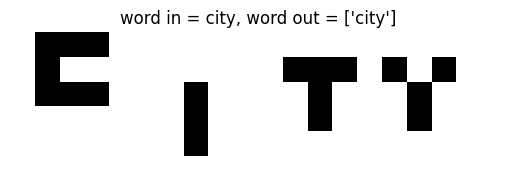
\includegraphics[width=14cm]{ex_5_6.png}
\end{center}
\caption{Example of the full model recognising the word "city".}
\end{figure}
\end{exa}

\section{Discussion}

\subsection{Model architecture}

The models in sections \ref{letters:letter}, \ref{letters:expand}, and \ref{letters:count} followed very intuitive architecture, where the weights for the convolutional kernels ended up looking like the letters they were trying to detect. This meant that the output node for each letter was activated when the kernels lined up with the corresponding letter in the grid.

The models in sections \ref{letters:words} and \ref{letters:alt} were far more challenging to develop by hand. The use of equation \ref{letters:eq1} seemed like a sensible starting point to indicate the values that we wished to bring forward and ultimately recognise as the output.

The GRU layers were particularly difficult to work with by hand. The original paper published by \citeauthor{DBLP:journals/corr/ChoMGBSB14} matches the Tensorflow implementation, where 
\begin{align*}
h_t = z_t \odot h_{t-1} + \left(1 - z_t\right) \odot \hat{h}_t.
\end{align*}
However, variations such as the minimal gated unit, proposed by \citet{heck2017simplified}, set
\begin{align*}
h_t = \left(1 - z_t\right) \odot h_{t-1} + z_t \odot \hat{h}_t.
\end{align*}
The latter is slightly more intuitive to work when working with $z_t \in \left\{0, 1\right\}$, as $z_t$ represents the condition for which we want to update the hidden state $h_t$, which would correspond to the outputs $x_t > 0$ which we are interested in. Overall, the network may have been slightly more efficient if we replaced $I\left(x_t > 0\right)$ with $I\left(x_t = 0\right)$. Similarly, when implementing equation \ref{bool:eq3} to create values to be used for $z_t$, it would have been possible to do this within the GRU layer using ReLU as the recurrent activation. This would slightly reduce the number of layers and overall weights in the model, although the GRU layers themselves would have been larger due to the increased number of inputs, therefore making this a difficult efficiency to implement with a limited familiarity with Python.

That being said, using the GRU layer in section \ref{letters:alt} provided a much more intuitive way to produce the sequence $\left\{\pmb{p}_t\right\}_{t=1}^{w_g}$ and was a worthwhile improvement to the first model.

\subsection{Possible improvements}

It is possible to reduce the architecture of the model significantly by using a larger GRU layer taking pairs $\left(x_t, I\left(x_t > 0\right)\right)$ as inputs. This solution would involve creating a hidden state of size $3w_g$, containing the output of length $w_g$ plus two copies of a similar vector to $\pmb{p}_t$ to keep track of the position. The position would be incremented using $I\left(x_t > 0\right)$ and the right-shift matrix as we have done in section \ref{letters:alt}. Two copies are stored in the hidden vector so that one of them can be multiplied by $x_t$ in the term $\left(\pmb{r_t} \odot \pmb{y}_{t-1}\right)$, allowing us to then propose $\hat{\pmb{y}}_{t}$ which contains $x_t$ right-shifted into the next available non-zero space in the output part of the hidden state, as well as the next position $\pmb{p}_t$. Overall, this would eliminate the need to create a "branch" in network architecture of the model to handle the positioning, as it is done within the GRU layer structure.


\chapter{O's and X's}

\section{Introduction}

This chapter will explore models that are designed to play O's and X's (or tic-tac-toe). We will represent the board using a $3 \times 3$ matrix for each of the 2 players. For each player, an entry of 0 represents a space where the player has not played a move, and an entry of 1 represents a space where the player has played a move. Denote a board $B$ as $B = \left\{\mathbf{X}_o, \mathbf{X}_x\right\}$, where $\mathbf{X}_o, \mathbf{X}_x \in M_{3,3}\left\{0,1\right\}$. Denote the starting board where all entries are 0 as $B_0$. Furthermore, let $\pmb{x}_p \in \left\{0,1\right\}^9$ denote the vector with the same entries as $\mathbf{X}_p$, in the following order:
\begin{align*}
    \begin{pmatrix}
        0 & 1 & 2 \\
        3 & 4 & 4 \\
        6 & 7 & 8 \\
    \end{pmatrix}.
\end{align*}

A game is played as follows. The board starts as $B = B_0$. Player $p$ selects an integer $i \in \left\{0, \dots, 8\right\}$ and updates the board $B$ by updating the $i$-th entry of $\pmb{x}_p$ from 0 to 1. The player $p$ then changes from $o$ to $x$ or vice versa.

A player $p$ wins if after the board $B$ is updated on their turn, they have a column, row, or diagonal consisting of three 1s in $\mathbf{X}_p$. In addition, if player $p$ selects $i$ where the $i$-th entry in $\pmb{x}_o$ or $\pmb{x}_x$ is 1 prior to updating $\pmb{x}_p$, then player $p$ loses. After 9 turns, if neither player has won or lost, the game is a draw.

This section will start with an experiment to see how effectively an ANN with dense layers can be trained to play O's and X's, and what seems to be the minimum requirements for a network to replicate perfect play. We will then repeat the experiment with an intuitive modification to the network architecture to help the network quickly reduce its rate of suggesting illegal moves.

\section{Methods}

The methods described in this section are implemented in the file \url{https://github.com/HectorLeitch/mas6041/blob/main/code/ox.py}.

\subsection{Creating a perfect player}

In O's and X's it is possible (for both players) to play a perfect game. The player who goes first playing perfectly is guaranteed not to lose. If the player going second also plays perfectly, the game will result in a draw; otherwise, the player going first may have the opportunity to win.

We can create a perfect player against which we can test the neural network players we create. The perfect player follows the algorithm proposed by \citep{crowley1993flexible}:

\begin{itemize}
    \item Win if possible: If a player has two in a row and the third position is available, play this position to win the game.
    \item Block opponent: If the opponent has two in a row and the third position is available, play this position to prevent the opponent winning the game.
    \item Fork: If there is a position available that creates two possibilities to play a win on the next turn, play this position.
    \item Block opponent's fork: If there is an available position such that the opponent could create a fork, play this position. If there are multiple positions, play a move that creates a possibility to play a win on the next turn, that is not blocked by one of the available forks to the opponent.
    \item Corner start: If it is the first move of the game, play in any corner position. This start can be ignored against a perfect player, but against an imperfect player it gives more chances for the opponent to make a mistake.
    \item Center: If the center position is available, play this position.
    \item Opposite corner: If the opponent has played in any corner and the opposite corner is available, play this position.
    \item Empty corner: If an empty corner position is available, play this position.
    \item Empty side: If an empty side position is available, play this position.
\end{itemize}

Furthermore, with this perfect player, we can generate training data by supplying it with board states and recording the suggested move as the response. We build a data set using the following assumptions:
\begin{itemize}
    \item The board state is one where it is the turn of the player who went first. As such we are teaching our networks exclusively to play first and draw or win only; they do not need to worry about reading the board and figuring out which player's turn it is.
    \item The board state is one which can only be reached through legal moves.
    \item The board state is not a finished game so there is at least one move that can be suggested.
\end{itemize}

This data set consists of 4519 separate states. Denote the set of board states as $\mathbf{B}$. We can think of our perfect player as a function $f_{\text{perfect}} : \mathbf{B} \rightarrow \left\{0, \dots, 8\right\}$, where $f_{perfect}\left(B\right)$ is the position from 0 to 8 suggested by the perfect player for any $B \in \mathbf{B}$.

Note that we have created the function to randomly select one of the four corners to start from so that more board states arise when testing the approximate models against the perfect player. This means that there are four possible entries for $f_{\text{perfect}}\left(B_0\right)$ in the training data which will depend on the random seed when the code is run, but the choice should not affect how the models train and ideally they should be able to handle board states that arise from any possible start.

\subsection{Approximate ANNs}

Our first goal is to build a model to approximate $f_{\text{perfect}}$ using two hidden dense layers, and an output layer (which is also a dense layer) with 9 outputs representing the choices from 0 to 8. Later on we will experiment with the number of nodes in each layer, so let the function representing the network approximating $f_{\text{perfect}}$ with $p$ and $q$ nodes in the first and second layers respectively be denoted as $f_{\left[p,q\right]}$.

We start by training a model with 20 nodes in each dense layer in order to establish suitable values for the training parameters: learning rate, epochs, and batch size. These values would then be reused while training models with varying numbers of nodes in each layer to establish roughly how well the model is able to perform with $p$ and $q$ nodes in the first and second layers respectively, and how small $p$ and $q$ can be reduced before the model starts to perform significantly worse than the perfect model.

The activation functions for all the approximate models are the ReLU function on the two dense layers, and the softmax function on the output layer. As such, $f_{\left[20,20\right]}$ will actually be a function from $\mathbf{B}$ to $\left(0, 1\right)^9$, where each output can be thought of as a probability or confidence in the corresponding position. We create a player by adding a classifier to the network that selects a position $i$ from $\left\{0, \dots, 8\right\}$ with probability $f_{\left[20,20\right]}\left(B\right)_i$, but this does not form part of the training.

In order to train the network weights we need a suitable loss function. The positions in the training data are one-hot encoded so each $\pmb{y}_i$ is a vector of length 9. The loss function is called categorical cross-entropy, and the total loss is calculated as
\begin{align*}
   L_{\text{cce}}\left(\pmb{y},\hat{\pmb{y}}\right) = - \sum_{i=1}^n \sum_{j=0}^9 y_{i,j} \log\left(\hat{y}_{i,j}\right).
\end{align*}

Within each $\pmb{y}_i$, only one entry will be 1 and the rest will be 0, so this loss can be thought of as trying to maximise the corresponding probability estimate in $\hat{\pmb{y}}_i$.

\subsection{Training procedure}\label{ox:train}

We will use Adam as the training optimizer, with a fixed learning rate that wa manually updated. The number of epochs and the batch size was also manually adjusted. An early stopping criteria monitoring the loss would stop training if no improvement was observed for 20 epochs.

As the goal was to find suitable values and not necessarily optimized values, a plot of the loss over time was created after each training run and the parameters were adjusted accordingly. This included whether or not the early stopping criteria had been met. Once it appeared that the values were suitable, the model was tested against a perfect player and a random player to verify that the approximation $f_{\left[20,20\right]}$ was close to $f_{\text{perfect}}$. A model was tested by tabulating the results of 100 games, recording whether any losses were due to illegal moves being suggested.

For a given set of training values, the shape of the plot provided guidance on how to adjust the parameters. Where the loss did not consistently decrease over time, showing a jagged shape on the graph with lots of increase and decreases, this indicated that the training process was struggling to find steps that resulted in decreasing the loss. This could suggest that the learning rate was too large, resulting in "over-shooting" when adjusting the weights and biases. Alternatively, this could also suggest that the batch size was not large enough, resulting in inaccurate estimates of the gradient descent direction. Conversely, where the shape of the graph was an extremely smooth decrease that continued all the way to the maximum number of epochs without triggering the stopping criteria, this meant that the model still required more epochs to finish training. This could suggest that the learning rate was too small, and a more appropriate learning rate would reduce the loss more efficiently.

In addition to choosing a moves from the values with probability proportional to the softmax outputs, we also can also test the models by changing the activation function on the final layer to argmax after training has been completed, so that the network chooses the position with the greatest output every time. This eliminates a lot of randomness and tends to yield much better approximations of $f_{\text{perfect}}$.

\subsection{Network size experiment}\label{ox:dense_ex}

Following the determination of the performance reached by the model with 20 nodes in each hidden layer, and experiment was run to reduce the size of the network and measure the impact to performance.

Models containing two hidden dense layers of size $p,q \in \left\{10, 11, \dots, 20\right\}$, where $p=q$, were trained using the parameters determined in the first part of the experiment. The models were tested by playing matches consisting of 100 games against the perfect player and the random player. Against the perfect player, the models were tested using the softmax and argmax position selectors. The intention behind this is to monitor the difference in softmax outputs if there are cases where the performance in the argmax models suddenly shifts after increasing or decreasing the network size by just one node per layer, to verify that there is a good reason behind a sudden shift.

\subsection{Residual connections}

We now introduce models with a new idea: \textit{residual connections}. A residual connection adds weights and biases that connect layers that are not adjacent to each other. The intuition behind adding these connections in this specific example is that it allows us to connect input positions directly to output positions, adding the option to include a penalty weight from positions that are occupied directly to the corresponding outputs. This should allow for models that are much better at avoiding illegal moves.

To show explicitly how this affects how the models are evaluated, note that the previous models would be evaluated as
\begin{align*}
    f_{\left[p,q\right]}\left(B\right) = \mathcal{L}^{\left[3\right]}\left( \mathcal{L}^{\left[2\right]}\left( \mathcal{L}^{\left[1\right]}\left(B\right)\right)\right).
\end{align*}

The model with residual connections is now evaluated as
\begin{align*}
    g_{\left[p,q\right]}\left(B\right) = \mathcal{L}^{\left[3\right]}\left( \mathcal{L}^{\left[2\right]}\left( \mathcal{L}^{\left[1\right]}\left(B\right)\right) + \mathbf{W}B + \pmb{b}\right)
\end{align*}
where $\mathbf{W}$ and $\pmb{b}$ are an additional weights matrix and bias vector.

As we have an idea of how the model with residual connections might use them, we will start by testing models with added penalty weights which the model is not allowed to train, and see if this helps the model learn values for the weights in the dense layers. If we consider the board $B$ to be $\left(\pmb{x}_o, \pmb{x}_x\right)^T$ then the weights matrix applying these penalties is
\begin{align*}
    \mathbf{W} = -20
    \begin{pmatrix}
        \mathbf{I}_{9} & \mathbf{I}_{9}
    \end{pmatrix},
\end{align*}
where $\mathbf{I}_9$ is the $9 \times 9$ identity matrix. We leave the bias as $\pmb{b} = \mathbf{0}$. With this addition, we repeat the experiment in section \ref{ox:dense_ex} starting by finding suitable training parameters, and training and testing models over varying sizes of dense layers. The range of layer sizes was kept the same for this experiment.

The final experiment in this chapter then repeats the process but allowing the model to also train the weights and biases of the residual connections. Based on the previous results we adjusted the range of sizes for this experiment, so that $p,q \in \left\{5, 6, \dots, 15\right\}$.


\section{Results}

The models described above are demonstrated in the Jupyter notebook \url{https://github.com/HectorLeitch/mas6041/blob/main/try_ox.ipynb}. The notebook is split into examples to demonstrate the code, which are described in the following paragraphs.


\begin{exa}
The function \verb|suggest_move(pq=, player=)| is the perfect player. This example simply shows the perfect player against itself, and against a random player. The function \verb|play_match(player_o=, player_x=, bestof=)| plays a match of \verb|bestof| games and records the results. This will be the basis of evaluating model performance in the following examples.

The code verifies that two perfect players draw against each other every time, and that the perfect player beats the random player overwhelmingly often; around 98\% of the time. These facts give us a quick way to evaluate how well an approximate model plays.
\end{exa}

\begin{exa}
The function \verb|make_simple_model(p=,q=,r=)| builds a model with \verb|p| and \verb|q| nodes in the first and second dense layers respectively, and sets the learning rate \verb|r| in the optimizer.

\begin{figure}[H]\label{ox:ex_6_1}
\begin{center}
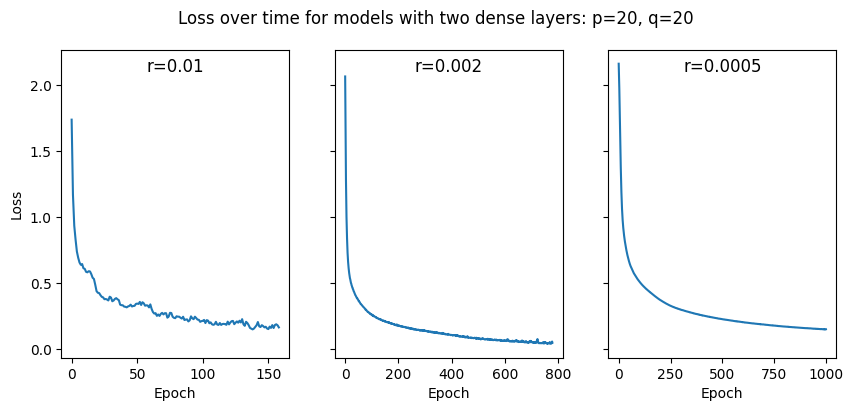
\includegraphics[width=14cm]{ex_6_1.png}
\end{center}
\caption{Loss over time for learning rates of 0.01, 0.002, and 0.0005. At 0.01, the steps struggle to consistently reduce the loss and training stops too early. At 0.0005, the loss is still decreasing by 1000 epochs. A learning rate of 0.02 is the "Goldilocks" value, reaching the stopping criteria at the lowest loss of the three models.}
\end{figure}

The model is trained with the function \verb|train_model_suggestions(M=,epochs=|
\verb|,batch_size=)| trains the model with the given parameters and returns the history of the loss over time, which can be plotted. Figure \ref{ox:ex_6_1} shows a collection of plots where models were trained for up to 1000 epochs with a batch size of 64.

The training parameters were adjusted as described in section \ref{ox:train} and a learning rate of 0.02 was chosen with a batch size of 64 and maximum number of epochs of 1000 to be the values for which to carry forward to training further models.
\end{exa}

\begin{exa}
Table \ref{ox:t1} shows the total number of draws, wins, and losses for each size of model in the three matches specified in section \ref{ox:dense_ex}, and the number of losses due to illegal moves. In some cases where the model using the softmax activation function on the output layer performs quite well, using the argmax activation function on the output layer instead leads to significantly better approximations of $f_{\text{perfect}}$ to the extent that they are able to draw every time against the perfect player.

\begin{table}[h!]
\centering
\begin{tabular}{ |c|c|c|c| }
 \hline
  vs. Player: & Perfect player & vs. Perfect player & vs. Random player \\
  Activation: & Softmax & Argmax & Argmax \\
  & D/W/L/I & D/W/L/I & D/W/L/I \\
 \hline
 10 & 42/0/58/40 & 100/0/0/0   & 25/63/12/6 \\
 11 & 27/0/73/43 & 0/0/100/100 & 16/71/13/7 \\
 12 & 44/0/56/24 & 0/0/100/0   & 10/85/5/3  \\
 13 & 67/0/33/11 & 100/0/0/0   & 19/78/3/0  \\
 14 & 34/0/66/66 & 0/0/100/100 & 14/85/1/0  \\
 15 & 50/0/50/39 & 0/0/100/100 & 9/91/0/0   \\
 16 & 77/0/23/16 & 100/0/0/0   & 27/71/2/0  \\
 17 & 39/0/61/4  & 0/0/100/0   & 20/74/6/0  \\
 18 & 72/0/28/27 & 100/0/0/0   & 9/91/0/0   \\
 19 & 60/0/40/40 & 100/0/0/0   & 13/87/0/0  \\
 20 & 95/0/5/5   & 100/0/0/0   & 3/97/0/0   \\
 \hline
 \multicolumn{4}{|c|}{D = Draws, W = Wins, L = Losses, I = Losses due to illegal moves} \\
 \hline
\end{tabular}
\caption{Full results table for models with two dense layers. The most difficult to explain behaviour is the losses using the argmax activation function, which are either all due to illegal moves or never due to illegal moves.}
\label{ox:t1}
\end{table}

The number of draws against the perfect player and wins against the random player is shown in figure \ref{ox:ex_6_2}. Against both the perfect player and the random player, it appears that the larger models may be performing slightly better.

 Figure \ref{ox:ex_6_3} shows the number of losses due to illegal moves in each match. It appears that in most cases, a loss is due to an illegal move. In the argmax models, it is not clear how some models lose all 100 games without any illegal moves.

The code in the notebook is able to repeat this experiment and the following two experiments with the user able to adjust the range of layer sizes tested.

\begin{figure}[H]\label{ox:ex_6_2}
\begin{center}
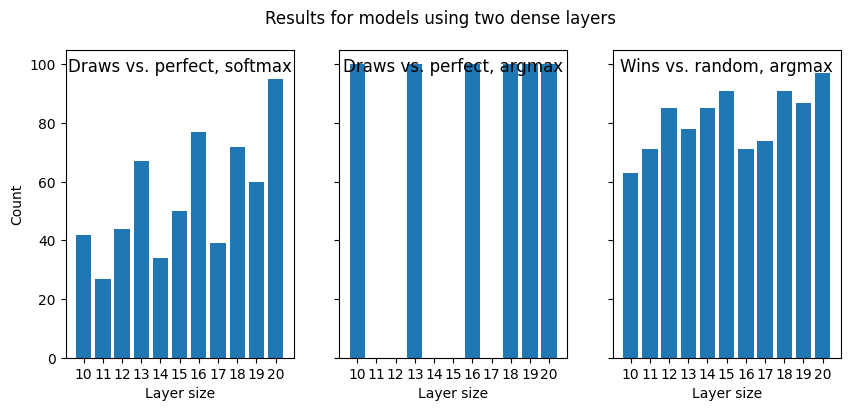
\includegraphics[width=14cm]{ex_6_2.png}
\end{center}
\caption{Larger models in general seem to be performing slightly better. There appear to be some potential outliers in the softmax models at sizes 13, 16, and 20.}
\end{figure}

\begin{figure}[H]\label{ox:ex_6_3}
\begin{center}
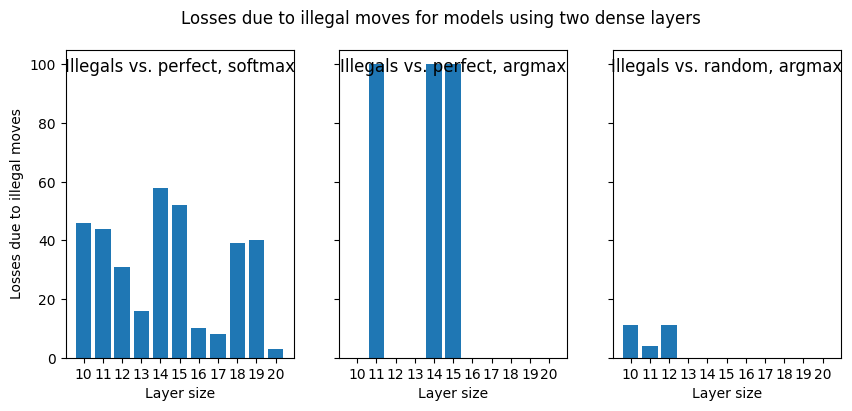
\includegraphics[width=14cm]{ex_6_3.png}
\end{center}
\caption{In most cases, models are losing due to illegal moves. Curiously this does not happen in all cases.}
\end{figure}
\end{exa}

\begin{exa}
Table \ref{ox:t2} shows the total number of draws, wins, and losses for each size of model using residual connections with the fixed weights, and the number of losses due to illegal moves. In comparison to table \ref{ox:t1}, we can see that the performance is much less affected by the size and in general the models perform very well. In particular, the performance of the models using the softmax activation function on the output layer is greatly increased with the weakest model still drawing 65\% of the time against the perfect player. This translates into all of the argmax models able to draw every time vs. the perfect player over the 100 games per match.

\begin{table}[h!]
\centering
\begin{tabular}{ |c|c|c|c| }
 \hline
  vs. Player: & Perfect player & vs. Perfect player & vs. Random player \\
  Activation: & Softmax & Argmax & Argmax \\
  & D/W/L/I & D/W/L/I & D/W/L/I \\
 \hline
 10 & 99/0/1/1   & 100/0/0/0 & 17/83/0/0 \\
 11 & 78/0/22/22 & 100/0/0/0 & 13/87/0/0 \\
 12 & 93/0/7/7   & 100/0/0/0 & 13/87/0/0 \\
 13 & 81/0/19/19 & 100/0/0/0 & 11/89/2/0 \\
 14 & 89/0/11/10 & 100/0/0/0 & 5/95/1/0  \\
 15 & 65/0/35/32 & 100/0/0/0 & 9/91/0/0  \\
 16 & 98/0/2/2   & 100/0/0/0 & 8/92/1/0  \\
 17 & 91/0/9/9   & 100/0/0/0 & 20/80/1/0 \\
 18 & 98/0/2/2   & 100/0/0/0 & 20/79/1/0 \\
 19 & 93/0/7/7   & 100/0/0/0 & 12/88/0/0 \\
 20 & 85/0/15/15 & 100/0/0/0 & 11/89/0/0 \\
 \hline
 \multicolumn{4}{|c|}{D = Draws, W = Wins, L = Losses, I = Losses due to illegal moves} \\
 \hline
\end{tabular}
\caption{Full results table for models with two dense layers and untrained residual connections. Here we see good performances from all the models and no sign that any of the models were too small. This informed the decision to alter the ranges for the final experiment in this chapter.}
\label{ox:t2}
\end{table}

\begin{figure}[H]\label{ox:ex_6_4}
\begin{center}
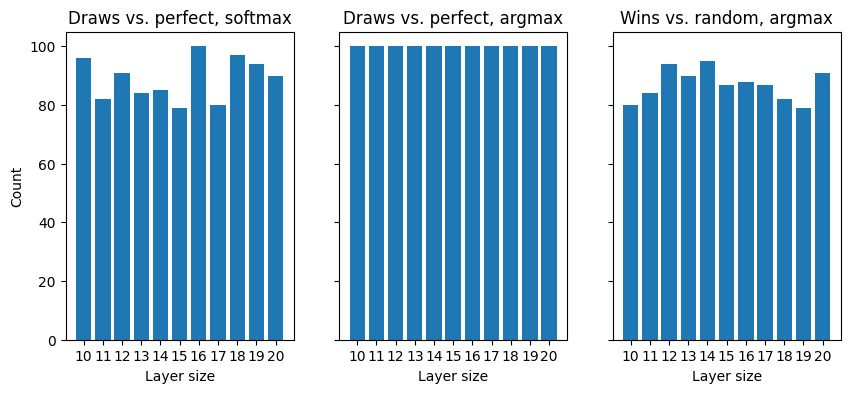
\includegraphics[width=14cm]{ex_6_4.png}
\end{center}
\caption{The difference in the overall level of performance from the models using residual connections is especially evident in this figure when compared to figure \ref{ox:ex_6_2}.}
\end{figure}

The number of draws against the perfect player and wins against the random player is shown in figure \ref{ox:ex_6_4}, where we can see the significant improvement in the models using the softmax activation function on the output layer compared to the models with only dense layers. From the graph we can also see that the performance appears to be more consistent across the range of layer sizes.

The code in the notebook is able to repeat this experiment with the user able to adjust the size of the penalty applied in the residual weights. If the results of the next example suggested it was necessary, this could have been re-adjusted from -20.
\end{exa}

\begin{exa}
Table \ref{ox:t3} shows the total number of draws, wins, and losses for each size of model using residual connections with the trainable weights, and the number of losses due to illegal moves. These models performed particularly well, and we adjusted the range of sizes to see if even smaller dense layers would affect the model performance. The results show that even with the model using just 5 nodes in each hidden layer and the softmax activation function on the output layer, the approximation to $f_{\text{perfect}}$ was very good. In particular, almost all cases of losing due to an illegal move have been eliminated.

\begin{table}[h!]
\centering
\begin{tabular}{ |c|c|c|c| }
 \hline
  vs. Player: & Perfect player & vs. Perfect player & vs. Random player \\
  Activation: & Softmax & Argmax & Argmax \\
  & D/W/L/I & D/W/L/I & D/W/L/I \\
 \hline
 5  & 83/0/17/0 & 100/0/0/0 & 14/86/0/0 \\
 6  & 83/1/16/0 & 100/0/0/0 & 18/80/2/0 \\
 7  & 96/0/4/0  & 100/0/0/0 & 21/79/0/0 \\
 8  & 99/0/1/0  & 100/0/0/0 & 19/81/0/0 \\
 9  & 94/0/6/0  & 100/0/0/0 & 27/73/0/0 \\
 10 & 87/0/13/5 & 100/0/0/0 & 19/80/1/0 \\
 11 & 98/0/2/1  & 100/0/0/0 & 22/74/4/0 \\
 12 & 99/0/1/0  & 100/0/0/0 & 11/88/1/0 \\
 13 & 92/0/8/0  & 100/0/0/0 & 15/84/1/0 \\
 14 & 98/0/2/2  & 100/0/0/0 & 12/88/0/0 \\
 15 & 94/0/6/1  & 100/0/0/0 & 10/88/2/2 \\
 \hline
 \multicolumn{4}{|c|}{D = Draws, W = Wins, L = Losses, I = Losses due to illegal moves} \\
 \hline
\end{tabular}
\caption{Full results table for models with two dense layers and trained residual connections. Overall the models perform extremely well, although they tended to draw more often against the random player than the models with untrained residual connections.}
\label{ox:t3}
\end{table}

The number of draws against the perfect player and wins against the random player is shown in figure \ref{ox:ex_6_6}. The notable features are that the models using the softmax activation function are performing even better than those shown in figure \ref{ox:ex_6_4}, but the models using the argmax activation function are not winning as often against the random player.

The code also shows that for the smallest of these models, the weights matrix did indeed learn to apply strong negative weights as our intuition suggested; these weights also confirm that the fixed penalty of -20 was a suitable value to use for the previous experiment. While most of the other weights were close to 0, many were of a reasonably large magnitude.

\begin{figure}[H]\label{ox:ex_6_6}
\begin{center}
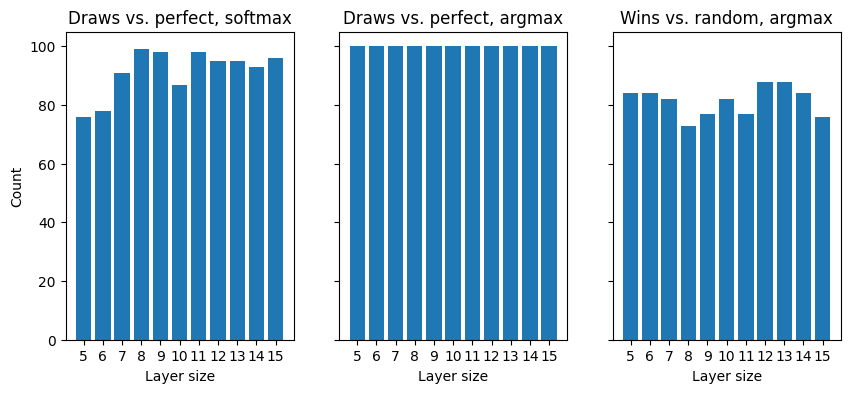
\includegraphics[width=14cm]{ex_6_6.png}
\end{center}
\caption{The stronger performance of the models using the softmax activation but weaker performance of the models using the argmax activation function suggests these models may have some particular bias towards moves that lead to draws.}
\end{figure}
\end{exa}

\section{Discussion}

\subsection{Interpretation of results}

The final part of the experiment where the models were allowed to train the weights and biases of the residual connections lead to models that performed very well despite a dramatic reduction in the number of available parameters compared to the models with no residual connections.

The model with $p=q=20$ and no residual connections had a total of $\left(18+1\right)*20+\left(20+1\right)*20+\left(20+1\right)*9=989$ parameters, whereas as the model with $p=q=5$ and trainable residual connections had a total of $\left(18+1\right)*5+\left(5+1\right)*5+\left(18+1\right)*9+\left(5+1\right)*9=350$ parameters.

It is worth noting that as we only trained one model at each size per variation, the numerical results may be quite unreliable. Particular models may have performed exceptionally well or poorly due to the initialization of the weights in the network. With more time, we could have trained multiple models at each size and measured their average performance. However, the magnitude of the difference supports the qualitative assessment that the residual connections lead to a great increase in performance and the ability to reduce the overall size of the network significantly.

\subsection{Training limitations}

This chapter consisted of experiments which involved training a collection of models. This was performed on a windows PC only using the CPU, and was therefore many times slower than it would have been with a dedicated GPU to accelerate the training. This motivated the decision to restrict the experiments to networks with two dense layers of equal size, as relaxing this constraint would have resulted in too many models to train in a reasonable time-frame. Accelerated training could have also allowed us to obtain more reliable data for the performance of models at each size as mentioned above.

\subsection{Further variations}

With more computing resources and time, it would have been interesting to see whether creating an imbalance in the layer sizes could improve the performance. Where the models were allowed to train the weights and biases of the residual connections, the performance appeared to be mainly driven by these weights and so it would have been interesting to see if dropping one of the hidden layers entirely would affect performance at all, and if near-perfect performance could still be reached, whether that would happen in a significantly shorter time.

\subsection{Reinforcement learning}

Reinforcement learning is a different approach to training models. Broadly speaking, this involves performing the task (i.e. playing a game of O's and X's) with an untrained model, and scoring each performance using a \textit{reward} or \textit{value} function. The model parameters are then adjusted and the process it iterated, with the goal being to maximize the reward. This allows us to train models without training data prepared, and also monitor how the model is learning to play the game as it trains. This was out of the scope of this project as reinforcement learning can be difficult to implement effectively.

\chapter{Digit recognition}

\section{Introduction}

The task of recognizing hand-written digits using neural networks, or other machine learning techniques, is a popular exercise. In particular the MNIST dataset of images of handwritten digits is a well-known dataset that has been used to develop convolutional neural networks \citep{ciresan2011convolutional} and support vector machines \citep{platt1998using}, among other machine learning techniques. In this chapter we will create both hand-built and trained neural networks to recognize digits, using a simplified dataset created by drawing pixels into a grid of $6 \times 6$ pixels.

The hand-built model uses a convolutional layer to identify certain types of pixels as features, which are then counted by another layer and passed to an output layer. Ideas seen in previous chapters are used again in this model. The trained model uses a smaller version of this architecture, and the goal is to try to identify parts of the hand-built model that can be used to enhance the performance of the trained model and increase the efficiency of the training process.

An image is represented by a matrix $\mathbf{X} \in M_{6,6}\left\{0,1\right\}$, where an entry of 1 represents a black pixel and a 0 represents a white pixel. A valid image containing a digit will have a corresponding label $y \in \left\{0, \dots, 9\right\}$. Each digit will be drawn using horizontal and vertical lines only, and will only be drawn in one "variation". Examples can be seen in figure \ref{digit:fig1}. There are some notable rules for certain digits, with the rest of the digits restricted by only using horizontal and vertical lines.

\begin{figure}[H]\label{digit:fig1}
\begin{center}
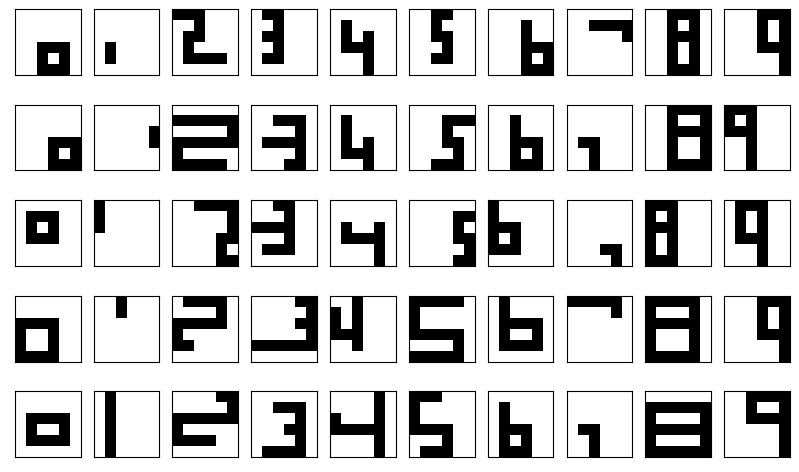
\includegraphics[width=12cm]{digit_1.png}
\end{center}
\caption{Examples of each digit. Notable rules are: 4s do not create a cross with the right vertical line; similarly 7s do not have a horizontal cross; 1s are a single vertical line with no bottom or top lines; 6s and 9s do not have a corner at the top and bottom respectively.}
\end{figure}

\section{Methods}

The methods described in this section are implemented in the file \url{https://github.com/HectorLeitch/mas6041/blob/main/code/digits.py}.

\subsection{Exact model}

Our first model is a hand-built exact model. This model uses similar ideas to the model created to recognize letters and words. In this case, each digit is broken down into a collection of pixel types that are recognized by convolution kernels applied to the input image, and then the collection of detected pixels of each type are combined to create the correct output.

The first layer of the neural network is a convolutional layer. There are 10 pixel types, shown in figure \ref{digit:fig2}, and so the layer has 10 channels, each with its own convolution kernel. There are three main types of pixels: pixel types 0 to 3 are line ends, pixel types 4 to 7 are corners, and pixel types 8 and 9 are the 'T junction' pixels. The assignment of a certain pixel to a particular type applies to the pixel in the middle of the $3 \times 3$ grid; as such, we need to design the kernels slightly differently to those in section \ref{letters:letter}, to account for possible variation in the surrounding pixels.

\begin{figure}[H]\label{digit:fig2}
\begin{center}
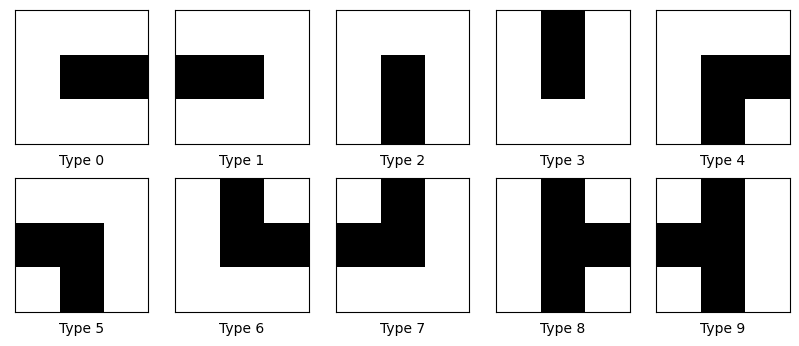
\includegraphics[width=12cm]{digit_2.png}
\end{center}
\caption{All 10 pixel types. Detection of these pixels will differ from in section \ref{letters:letter}, so these should not be thought of as representations of the convolution kernels.}
\end{figure}

The convolution kernels are matrices in $M_{3,3}\left\{-1,0,1\right\}$. A 1 is placed in the black positions in figure \ref{digit:fig2}, corresponding to the pixels we expect to find a value of 1 in for each type. A 0 is placed in positions where we may or may not find a value of 1 in the image. For example, a pixel of type 0 could be found in the image as any member of the set
\begin{align*}
    \left\{
    \begin{pmatrix}
        0 & 0 & 0 \\
        0 & 1 & 1 \\
        0 & 0 & 0
    \end{pmatrix},
    \begin{pmatrix}
        0 & 0 & 1 \\
        0 & 1 & 1 \\
        0 & 0 & 0
    \end{pmatrix},
    \begin{pmatrix}
        0 & 0 & 0 \\
        0 & 1 & 1 \\
        0 & 0 & 1
    \end{pmatrix},
    \begin{pmatrix}
        0 & 0 & 1 \\
        0 & 1 & 1 \\
        0 & 0 & 1
    \end{pmatrix}
    \right\}.
\end{align*}
Similarly, a -1 is placed in positions where a value of 1 in the image would mean that the pixel is of a different type. So even though the matrix
\begin{align*}
    \begin{pmatrix}
        0 & 1 & 0 \\
        0 & 1 & 1 \\
        0 & 0 & 0
    \end{pmatrix}
\end{align*}
contains the pixels for a type 0 pixel, the value of 1 in the top middle position means it is a type 6 pixel. Letting $\mathbf{K}_i$ denote the convolution kernel that detects pixel type $i$, the full list of convolution kernels in the first layer is as follows:
\begin{center}
\begin{tabular}{c c}
    $\mathbf{K}_0 =
    \begin{pmatrix}
        -1 & -1 & 0 \\
        -1 &  1 & 1 \\
        -1 & -1 & 0
    \end{pmatrix}$ &
    $\mathbf{K}_1 =
    \begin{pmatrix}
         0 & -1 & -1 \\
         1 &  1 & -1 \\
         0 & -1 & -1
    \end{pmatrix}$ \\
    $\mathbf{K}_2 =
    \begin{pmatrix}
        -1 & -1 & -1 \\
        -1 &  1 & -1 \\
         0 &  1 &  0
    \end{pmatrix}$ &
    $\mathbf{K}_3 =
    \begin{pmatrix}
         0 &  1 &  0 \\
        -1 &  1 & -1 \\
        -1 & -1 & -1
    \end{pmatrix}$ \\
    $\mathbf{K}_4 =
    \begin{pmatrix}
        -1 & -1 &  0 \\
        -1 &  1 &  1 \\
         0 &  1 & -1
    \end{pmatrix}$ &
    $\mathbf{K}_5 =
    \begin{pmatrix}
         0 & -1 & -1 \\
         1 &  1 & -1 \\
        -1 &  1 &  0
    \end{pmatrix}$
\end{tabular}
\begin{tabular}{c c}
    $\mathbf{K}_6 =
    \begin{pmatrix}
         0 &  1 & -1 \\
        -1 &  1 &  1 \\
        -1 & -1 &  0
    \end{pmatrix}$ &
    $\mathbf{K}_7 =
    \begin{pmatrix}
        -1 &  1 &  0 \\
         1 &  1 & -1 \\
         0 & -1 & -1
    \end{pmatrix}$ \\
    $\mathbf{K}_8 =
    \begin{pmatrix}
        0 & 1 & 0 \\
        0 & 1 & 1 \\
        0 & 1 & 0
    \end{pmatrix}$ &
    $\mathbf{K}_9 =
    \begin{pmatrix}
        0 & 1 & 0 \\
        1 & 1 & 0 \\
        0 & 1 & 0
    \end{pmatrix}$
\end{tabular}
\end{center}

Similar to section \ref{letters:letter}, and specifically equation \ref{letters:eq0}, the convolution kernel weights are combined with a bias and ReLU activation function, so that the output in channel $i$ for a particular pixel is 1 if the pixel is of type $i$ and 0 otherwise. The biases are determined in the same way as the number of 1s in the kernel, minus one. This gives the bias vector
\begin{align*}
    \pmb{b}_1 =
    \begin{pmatrix}
        -1 & -1 & -1 & -1 & -2 & -2 & -2 & -2 & -3 & -3
    \end{pmatrix}.
\end{align*}

Finally, there is zero-padding applied to the input in the first convolutional layer, so that the output for each channel is a feature map that is also size $6 \times 6$.

The second layer of the model counts the number of occurrences of each pixel type. This is enough to distinguish every digit apart from 2 and 5, which both have one pixel of type 0, 1, 4, 5, 6, and 7. To distinguish 2 and 5, the model must evaluate the relative positions of the pixels of type 4, 5, 6, and 7. While the feature map could be flattened into a 10 vectors of length 36, and provided to a dense layer to perform this step, it is more convenient to use another convolutional layer with a $6 \times 6$ kernel for each channel. With no zero-padding, this results in a single output per channel, 10 of which are the counts for the pixel types.

In total, the second layer has 17 output channels. The output of the first layer has 10 channels, so we need to assign the weights for 170 kernels of size $6 \times 6$. For the channel corresponding to the detection of pixel type $i \in \left\{0, \dots, 9\right\}$, the $i$-th kernel will be set to a $6 \times 6$ matrix of ones $\mathbf{1}_{6,6}$ and the other channels will be set to a $6 \times 6$ matrix of zeros $\mathbf{0}_{6,6}$. This counts the number of detected pixels in each channel from the first layer.

The kernels that determine the positions of pixels of type 4, 5, 6, and 7, are based on the matrix
\begin{align*}
    \mathbf{H} =
    \begin{pmatrix}
        0 & 0 & 0 & 0 & 0 & 0 \\
        1 & 1 & 1 & 1 & 1 & 1 \\
        2 & 2 & 2 & 2 & 2 & 2 \\
        3 & 3 & 3 & 3 & 3 & 3 \\
        4 & 4 & 4 & 4 & 4 & 4 \\
        5 & 5 & 5 & 5 & 5 & 5 \\
    \end{pmatrix}.
\end{align*}
For digits 2 and 5, the first layer of the model detects one pixel of types 0, 1, 4, 5, 6, and 7. For the feature channels that contain the detected type 4, 5, 6, and 7 pixels, multiplying the feature output by $\mathbf{H}$ element-wise returns the number of pixels from the top that the pixel is on, and similarly multiplying the feature output by $\mathbf{H}^T$ element-wise returns the number of pixels from the left that the pixel is on.

A 2 will be indicated by the pixels of type 4 and 6 appearing below the pixels of type 5 and 7, and conversely a 5 will be indicated by the pixels of type 4 and 6 appearing above the pixels of type 5 and 7. We also need to check that the pixels of type 4 and 6 are vertically aligned, and the pixels of type 5 and 7 are vertically aligned. Creating indicators for these conditions ensures that digits 2 and 5 will be detected, and the model is also able to reject configurations such as the one shown in figure \ref{digit:fig3}.

\begin{figure}[H]\label{digit:fig3}
\begin{center}

\includegraphics[width=6cm]{digit_3.png}
\end{center}
\caption{This configuration has the heights of the pixels of type 4 and 6 equal to the heights of pixels of type 5 and 7 respectively. The pixels of type 4 and 5 could be raised or lowered, so we need to check this shape is not present by confirming the vertical alignment of the pixels instead.}
\end{figure}

Let $h_p$ and $w_p$ be the number of pixels that the detected pixel of type $p$ is from the top and left respectively (noting that an increase in $h_p$ indicates the pixel is lower in the image), obtained by multiplying the corresponding feature output by $\mathbf{H}$ and $\mathbf{H}^T$. We now re-purpose equation \ref{letters:eq1} with these values to create the required indicators. We have
\begin{align*}
    I\left(h_4 + h_6 > h_5 + h_7\right) &= \left(h_4 + h_6 - h_5 - h_7\right)_+ - \left(h_4 + h_6 - h_5 - h_7 - 1\right)_+, \\
    I\left(h_5 + h_7 > h_4 + h_6\right) &= \left(h_5 + h_7 - h_4 - h_6\right)_+ - \left(h_5 + h_7 - h_4 - h_6 - 1\right)_+, \\
    I\left(w_4 = w_6\right) &= \left(w_4 - w_6 + 1\right)_+ - 2\left(w_4 - w_6\right)_+ + \left(w_4 - w_6 - 1\right)_+.
\end{align*}
Evaluating these in the output layer requires 7 extra channels in the second layer. The kernels corresponding to the feature output for the pixel of type $p$ are set to $\pm \mathbf{H}$ or $\pm \mathbf{H}^T$ depending on whether the coefficient for each $h_p$ or $w_p$ is 1 or -1 in the corresponding component. A bias of 1 or -1 is added to complete these terms. All other weights and biases are set to 0. The ReLU activation function is then applied to the layer as a whole to create the components of the indicators above; the counts in the first 10 channels are unaffected by this.

The output layer is a dense layer which again functions using a variation of equation \ref{letters:eq0}. There are 10 outputs corresponding to each digit from 0 to 9; the weights for each digit are 1 where the pixel types are expected to be detected, and -1 where they are not. From indicator component channels of the second layer, the weights are 0 apart from to the outputs corresponding to 2 and 5, where the weights are assigned to construct the indicators that should be true for each output. For a digit 2, we should have
\begin{align*}
    I\left(h_4 + h_6 > h_5 + h_7\right) &= 1, \\
    I\left(h_5 + h_7 > h_4 + h_6\right) &= 0, \\
    I\left(w_4 = w_6\right) &= 1,
\end{align*}
and for a digit 5, we should have
\begin{align*}
    I\left(h_4 + h_6 > h_5 + h_7\right) &= 0, \\
    I\left(h_5 + h_7 > h_4 + h_6\right) &= 1, \\
    I\left(w_4 = w_6\right) &= 1,
\end{align*}

The bias for each output is the negative of the number of ones in the weights corresponding to each output, minus one. The bias vector is therefore
\begin{align*}
    \pmb{b_3} =
    \begin{pmatrix}
        -3 & -1 & -7 & -5 & -4 & -6 & -4 & -2 & -5 & -4
    \end{pmatrix}.
\end{align*}

The ReLU activation function is applied to the result, so that the output of this layer when a digit is present is the one-hot encoding representing the detected digit, and if no digit is present the output is a vector of zeroes $\mathbf{0}_{10}$.

\subsection{Approximate ANNs}

We now create an approximate model that can be trained using the dataset containing all the possible images containing digits. The model uses the same architecture in terms of the layer types and their activation functions, but the convolutional layers only have 3 channels each. If a model can achieve perfect performance on the training data, we are able to investigate the final weights in visualizations using colours, or 3-channel red/green/blue (RGB) values.

The process for finding suitable training values closely followed the process previously described in section \ref{ox:train}. However, it was found that experimenting with the \textit{patience}, the number of epochs over which no improvement would cause training to stop early, was necessary due some of the common behaviour found with this network architecture and training data. The parameters were adjusted by examining plots of the loss over time, and values were chosen once we were able to reliably train a model with satisfactory performance.

The model performance for the approximate models was assessed by counting the number or percentage of correct classifications made on the dataset containing all the possible images containing digits, ignoring any further images that did not contain digits.

\subsection{Improving ANNs}

The goal of the models created in this section was to improve the stability of the training and the overall improvement of the approximate ANNs. The strategy implemented was to repeat the training process with the established parameters, but initializing the weights and biases of the first convolutional layer using the weights and biases from the first layer of the hand-built exact model, corresponding to a subset of the channels.

As there are $10^3$ combinations of selections we can make to initialize the weights, it was impractical to run an experiment that tested training at least one model using each selection. Therefore, we chose to experiment with a smaller subset. Five models were trained where the weights and biases for the first layer were initialized using three copies of the kernel and bias used to detect each pixel type from the hand-built exact model. This resulted in 50 total models trained, which did not take an excessive amount of time to run.

If it made sense to do so, we could have extended this experiment by repeating the experiment, but only using two copies of each kernel while fixing the third kernel to be the one that achieved the best performance in the first round of tests. A final round of tests using the best two-kernel selection from the second round would give us a selection of three starting kernels that we believe to be among the best possible using this idea. However, the results proved that only the first round of tests was necessary to achieve a satisfactory improvement in performance.

\section{Results}

The models described above are demonstrated in the Jupyter notebook \url{https://github.com/HectorLeitch/mas6041/blob/main/try_digits.ipynb}. The notebook is split into examples to demonstrate the code, which are described in the following paragraphs.

\begin{exa}
The function \verb|make_exact_model()| creates the hand-built model which takes an input $\mathbf{X} \in M_{6,6}\left\{0,1\right\}$ and returns the one-hot representation of a recognized digit, or a vector of 0s if no digit is detected. The function \verb|model_classify(M=, img=)| shows the output for the model \verb|M| evaluated on the image \verb|img| as an integer, or shows "reject" if no digit is found.

The example code shows the model working on individual random images, and a selection of images without digits in them to show that it properly rejects certain cases. The function \verb|check_model()| evaluates the model on the full set of possible inputs containing digits, showing that it is correct in every case.
\end{exa}

\begin{exa}
The function \verb|make_approx_model(p=3, q=3, r=)| creates an approximate model sharing the same layer architecture as the exact model, but with $p=q=3$ channels in the convolutional layers. The function \verb|train_approx|\\ \verb|_model(M=, epochs=, batch_size=, patience=)| implements the training of the model, with the training parameters free to be modified.

\begin{figure}[H]\label{digit:ex_7_1}
\begin{center}
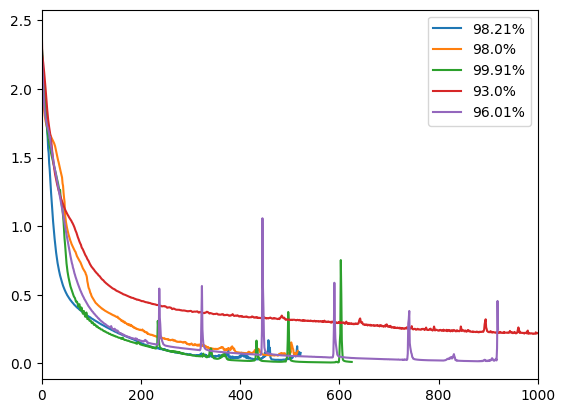
\includegraphics[width=12cm]{ex_7_1.png}
\end{center}
\caption{Loss over time for five models using the same values for the training parameters; the differences are therefore due to the random initialization. There is a reasonable variety in how many epochs were needed, with one run not meeting the early stopping criteria and performing noticeably worse.}
\end{figure}

It was found that the training of this model was quite sensitive to the random initialization of the weights. Figure \ref{digit:ex_7_1} shows the loss over time for five different runs using the same values for the training parameters: the learning rate was set to 0.003, and the values for epochs, batch size, and patience were 1000, 128, and 40 respectively. Furthermore, figure \ref{digit:ex_7_2} shows the kernels for the first layer after training. It can be seen that there is no clear pattern in how the first layer is creating features.

However, with the training parameters set these values, quite strong performance could be reliably achieved with the models tending to classify >96\% of the inputs correctly. This was deemed satisfactory performance to use these values for the training parameters going forward.

\begin{figure}[H]\label{digit:ex_7_2}
\begin{center}
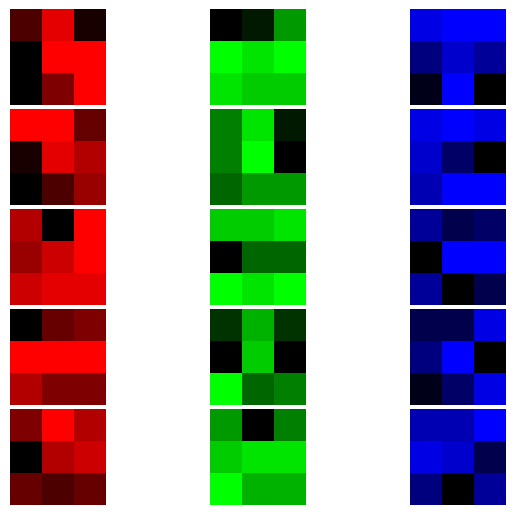
\includegraphics[width=6cm]{ex_7_2.png}
\end{center}
\caption{Kernels for the first layer in each trained model. Each of the five models occupies one row. While some of the kernels resemble the ones we used to detect certain pixels, there doesn't seem to be a clear pattern to how the first layer is creating features.}
\end{figure}
\end{exa}

\begin{exa}
The function \verb|test_starting_kernels(sk=, r=, epochs=,| \\ \verb|batch_size=, patience=)| creates an approximate model sharing the same layer architecture as the exact model, but with $p=q=3$ channels in the convolutional layers. It then initializes the kernel weights in the first layer using the kernels used to detect pixels types corresponding to the types listed in the \verb|sk| parameter. The model is then trained using the values for the training parameters chosen from the previous example.

\begin{figure}[H]\label{digit:ex_7_3}
\begin{center}
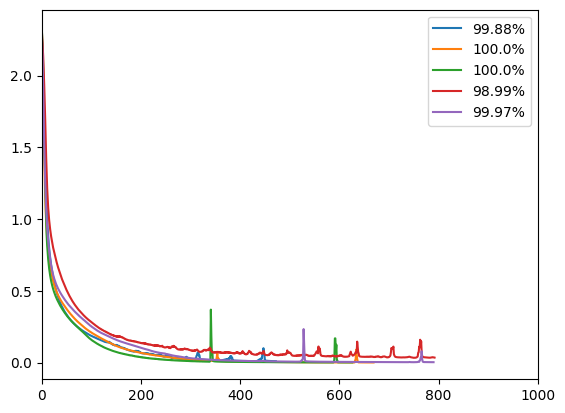
\includegraphics[width=10cm]{ex_7_3.png}
\end{center}
\caption{Loss over time for five models, starting with kernels $\mathbf{K}_0$, $\mathbf{K}_6$, and $\mathbf{K}_9$. The stability of the training procedure has been vastly improved and the performance of the models is very strong, sometimes resulting in a 100\% score. Note that the choice of starting kernels was arbitrary, and the code can be used to demonstrate that these  results are quite typical for many combinations.}
\end{figure}

It was found that using virtually any combination of starting kernels resulted in a much more stable training procedure, with stronger end results than the models trained from randomly initialized weights. Figure \ref{digit:ex_7_3} shows the loss over time for five models, starting with kernels $\mathbf{K}_0$, $\mathbf{K}_6$, and $\mathbf{K}_9$.

We can also see that there is a clear pattern in the final kernels in the first layer after training in figure \ref{digit:ex_7_4}.

\begin{figure}[H]\label{digit:ex_7_4}
\begin{center}
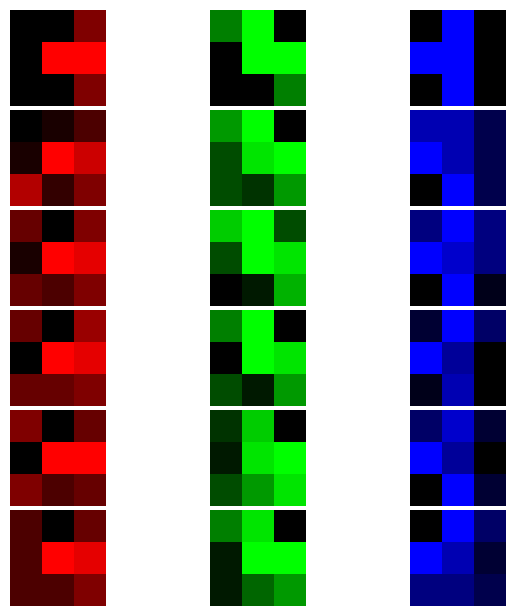
\includegraphics[width=6cm]{ex_7_4.png}
\end{center}
\caption{Kernels for the first layer in each trained model, starting with kernels $\mathbf{K}_0$, $\mathbf{K}_6$, and $\mathbf{K}_9$. Here we can see that the starting kernel is often clearly visible in its corresponding final kernel. The first row shows the starting kernels for this selection of models.}
\end{figure}

The fact that the kernels in the first layer still resemble the starting kernel for each channel, and consistently do so, is in correlation with the improved stability of the training procedure and performance of the resulting models.
\end{exa}

\begin{exa}
The function \verb|test_all(),| performs the experiment of comparing the training of models using three copies of the kernel used to detect each pixel type as initialized weights for the first layer. Table \ref{digit:t1} shows the tabulated results of the choice of starting kernel against the mean percentage of the inputs that were correctly classified across the five models.

Figure \ref{digit:ex_7_5} shows the kernels for the first layer of each model after training for the models using $\mathbf{K}_9$ as the starting kernel. Interestingly, there appears to be more deviation from the starting kernel in this case, which could be due to using three copies in the initialization. While the choice of kernel was sensitive to the random seed, this behaviour was observed consistently rerunning the experiment using the notebook.

\begin{table}[h!]
\centering
\begin{tabular}{ |c|c| }
 \hline
  Starting kernel & Correct classifications (\%) \\
 \hline
 $\mathbf{K}_0$ & 97.79 \\
 $\mathbf{K}_1$ & 98.00 \\
 $\mathbf{K}_2$ & 99.85 \\
 $\mathbf{K}_3$ & 99.69 \\
 $\mathbf{K}_4$ & 99.92 \\
 $\mathbf{K}_5$ & 98.72 \\
 $\mathbf{K}_6$ & 99.72 \\
 $\mathbf{K}_7$ & 99.40 \\
 $\mathbf{K}_8$ & 99.48 \\
 $\mathbf{K}_9$ & 99.99 \\
 \hline
\end{tabular}
\caption{Results for each choice of starting kernel. Many of the choices averaged close to 100\% correctness and while $\mathbf{K}_9$ was the best performer, variation in the initialization of the weights and biases in the other layers account for the difference. Rerunning this test with a different seed can produce a different result.}
\label{digit:t1}
\end{table}

\begin{figure}[H]\label{digit:ex_7_5}
\begin{center}
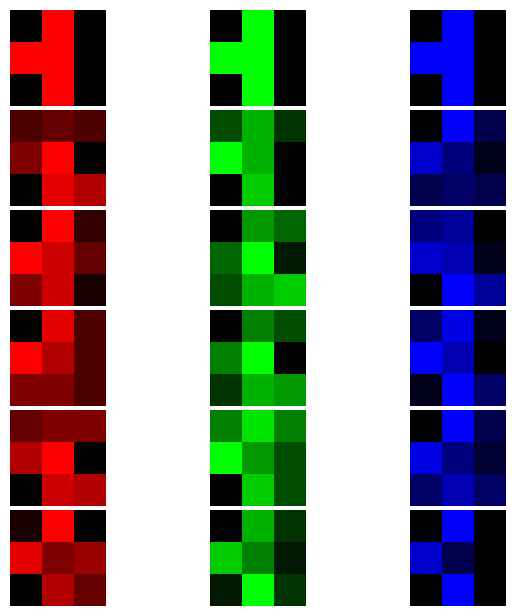
\includegraphics[width=6cm]{ex_7_5.png}
\end{center}
\caption{Kernels for the first layer in each trained model, starting with kernels $\mathbf{K}_0$, $\mathbf{K}_6$, and $\mathbf{K}_9$. Here we can see that the starting kernel is often clearly visible in its corresponding final kernel.}
\end{figure}
\end{exa}

\section{Discussion}

\subsection{Model architecture}

The exact model in this chapter followed a similar design philosophy to the letter and word detection, where the first convolution layer is designed with kernels matching the structure of the pixels they are intended to detect, with the biases and ReLU activation function restricting the outputs to $\left\{0,1\right\}$. The designs in this chapter required a little more thought as it was possible that pixels of certain types could be next to each other within a $3 \times 3$ space.

\subsection{Training behaviour}

The approximate models in this chapter proved slightly more challenging to train than those in previous chapters. Initially, the trained models seemed to be highly sensitive to the initialization of the weights and biases. Adjusting the learning rate and batch size was quite difficult as large spikes where the loss increased were frequently observed; this may have affected whether or not the stopping criteria was met, so this motivated the decision to add the patience to the stopping criteria as a parameter in an attempt to minimize the impact of a sudden increase in the loss.

The models using fixed kernels suffered much less from these issues. It is possible that in choosing weights and biases that were much better than randomly chosen ones, the model trained as if it had fewer parameters in the model. A possible extension to the experiments performed would have been to not let the model train the weights and biases in the first layer and see if this limited the performance, in a similar fashion to what was done with the residual connections in the previous chapter. However, as the final models chosen in the final part of the experiment were often able to reach 100\% accuracy, it was decided to spend more time on the other chapters in this project.


\chapter{Conclusion}

\section{Summary of completed work}

The overall goal of this project was to use small neural networks to tackle a variety of problem scenarios, with a focus on using the design of the network architecture to yield models that worked in a way that could be understood by the user, and were less of a "black box" compared to traditional deep neural networks trained on large datasets. Chapters 2 to 5 were mainly focused on building neural networks by hand to achieve a specific task. In some cases, the initial model could be improved upon on generalized. Chapters 6 and 7 mainly focused on training neural networks for slightly more complex tasks, and adapting the network architecture in an intuitive fashion to try to improve the model performance. The models were demonstrated using Jupyter notebooks, each supported by custom functions written in a source file, that can be downloaded and modified to verify the robustness of the models and explore the networks in detail.

\section{Discussion}

Each chapter contains its own discussion of particular items of interest that arose working on the corresponding problems. However, there were a few common themes which are worth highlighting.

From the chapters involving hand-built models, it became clear that where the input domain was restricted to matrices or vectors of integers, a good strategy was to use weights and biases that were also integers. This restricted the domain at each layer to vectors or matrices of integers only, allowing key results such as equations \ref{bool:eq5}, \ref{letters:eq0}, and \ref{letters:eq1} to be applied. The ReLU activation function was the obvious choice to pair with these designs to increase the capabilities of certain layers, as it introduced a further restriction to non-negative integers. The main challenge in developing these models was implementing them in Tensorflow/Keras, where it became difficult to ensure the size and dimensions of each tensor object was correct.

From the chapters involving trained models, the adaptations to the model architectures were generally successful in achieving their goal of improving the model performance. The models were often able to achieve 100\% accuracy with relatively little training after improvements, depending on the random seed set in the program. This was certainly a success according to the original aims of the project, as it was demonstrated that the improvements came from changing the network architectures rather than modifying the training process. However, the ability to accurately and reliably quantify the improvements in each scenario was restricted by the available computing resources and time.

\section{Further work}

The work done in each chapter tackled each problem from scratch, and therefore we have discussed possible extensions or improvements to the work that directly follow the work done in each case. It is also possible that some of the findings in this project could be more generally applied to other problems. There seems to be little research published regarding small neural networks in particular, so it is possible that continuing to expand these examples would provide useful findings for designing and optimizing smaller networks.

The design of a neural network architecture is a process itself that can be automated and tackled using a machine learning-based approach. \citet{luo2018neural} and \citet{pham2018efficient} propose algorithms for efficiently optimizing the architecture of a network through exploring an \textit{architecture space}. The results of chapters 6 and 7 suggest that for specific problems, particular choices could be made to steer the optimization of a neural network architecture through reducing this architecture space, based on a human's understanding of the specific problem.



\newpage
References to get:
python packages:
keras
tensorflow
numpy
itertools
matplotlib



% To amend the appendices, edit (and save) the file
% in the current directory called appendices.tex and
% then recompile this file using pdflatex.

\include{appendices}

%%%%%%%%%%%%%%%%%%%%%%%%%%%%%%%%%%%%%%%%%%%%%%%%%%%%
% To add to or change the References, edit (and save)
% the file called references.tex in the current
% directory and then recompile this file using pdflatex.
%If the file compiles but leaves a question mark where
%you expect to see a reference, recompile using bibtex
%and then recompile using pdflatex again.
% Do not change any code below here.
%%%%%%%%%%%%%%%%%%%%%%%%%%%%%%%%%%%%%%%%%%%%%%%%%%%%

\backmatter
\renewcommand{\bibname}{References}
\bibliography{references}
\bibliographystyle{apalike}

%%%%%%%%%%%%%%%%%%%%%%%%%%%%%%%%%%%%%%%%%%%%%%%%%%%%
%%%%%%%%%%%%%%%%%%%%%%%%%%%%%%%%%%%%%%%%%%%%%%%%%%%%

\end{document}
